\documentclass[11pt,a4paper, d]{scrartcl}
    \usepackage[scaled]{helvet}
    \usepackage{fancyhdr}
    \usepackage{amsmath}
\usepackage{amsthm}
\usepackage{amssymb}
\usepackage{amsfonts}
    \usepackage[breakable]{tcolorbox}
    \usepackage{parskip} % Stop auto-indenting (to mimic markdown behaviour)

    \usepackage{parskip} % Stop auto-indenting (to mimic markdown behaviour)
    
    \usepackage{iftex}
    \ifPDFTeX
    	\usepackage[T1]{fontenc}
    	\usepackage{mathpazo}
    \else
    	\usepackage{fontspec}
    \fi

    % Basic figure setup, for now with no caption control since it's done
    % automatically by Pandoc (which extracts ![](path) syntax from Markdown).
    \usepackage{graphicx}
     \graphicspath{{figures/}{RareEvent/figures/}}
    % Maintain compatibility with old templates. Remove in nbconvert 6.0
    \let\Oldincludegraphics\includegraphics
    % Ensure that by default, figures have no caption (until we provide a
    % proper Figure object with a Caption API and a way to capture that
    % in the conversion process - todo).
    \usepackage{caption}
    \DeclareCaptionFormat{nocaption}{}
    \captionsetup{format=nocaption,aboveskip=0pt,belowskip=0pt}

    \usepackage{float}
    \floatplacement{figure}{H} % forces figures to be placed at the correct location
    \usepackage{xcolor} % Allow colors to be defined
    \usepackage{enumerate} % Needed for markdown enumerations to work
    \usepackage{geometry} % Used to adjust the document margins
    \usepackage{amsmath} % Equations
    \usepackage{amssymb} % Equations
    \usepackage{textcomp} % defines textquotesingle
    % Hack from http://tex.stackexchange.com/a/47451/13684:
    \AtBeginDocument{%
        \def\PYZsq{\textquotesingle}% Upright quotes in Pygmentized code
    }
    \usepackage{upquote} % Upright quotes for verbatim code
    \usepackage{eurosym} % defines \euro
    \usepackage[mathletters]{ucs} % Extended unicode (utf-8) support
    \usepackage{fancyvrb} % verbatim replacement that allows latex
    \usepackage{grffile} % extends the file name processing of package graphics 
                         % to support a larger range
    \makeatletter % fix for old versions of grffile with XeLaTeX
    \@ifpackagelater{grffile}{2019/11/01}
    {
      % Do nothing on new versions
    }
    {
      \def\Gread@@xetex#1{%
        \IfFileExists{"\Gin@base".bb}%
        {\Gread@eps{\Gin@base.bb}}%
        {\Gread@@xetex@aux#1}%
      }
    }
    \makeatother
    \usepackage[Export]{adjustbox} % Used to constrain images to a maximum size
    \adjustboxset{max size={0.9\linewidth}{0.9\paperheight}}

    % The hyperref package gives us a pdf with properly built
    % internal navigation ('pdf bookmarks' for the table of contents,
    % internal cross-reference links, web links for URLs, etc.)
    \usepackage{hyperref}
    % The default LaTeX title has an obnoxious amount of whitespace. By default,
    % titling removes some of it. It also provides customization options.
    \usepackage{titling}
    \usepackage{longtable} % longtable support required by pandoc >1.10
    \usepackage{booktabs}  % table support for pandoc > 1.12.2
    \usepackage[inline]{enumitem} % IRkernel/repr support (it uses the enumerate* environment)
    \usepackage[normalem]{ulem} % ulem is needed to support strikethroughs (\sout)
                                % normalem makes italics be italics, not underlines
    \usepackage{mathrsfs}
    

    
    % Colors for the hyperref package
    \definecolor{urlcolor}{rgb}{0,.145,.698}
    \definecolor{linkcolor}{rgb}{.71,0.21,0.01}
    \definecolor{citecolor}{rgb}{.12,.54,.11}

    % ANSI colors
    \definecolor{ansi-black}{HTML}{3E424D}
    \definecolor{ansi-black-intense}{HTML}{282C36}
    \definecolor{ansi-red}{HTML}{E75C58}
    \definecolor{ansi-red-intense}{HTML}{B22B31}
    \definecolor{ansi-green}{HTML}{00A250}
    \definecolor{ansi-green-intense}{HTML}{007427}
    \definecolor{ansi-yellow}{HTML}{DDB62B}
    \definecolor{ansi-yellow-intense}{HTML}{B27D12}
    \definecolor{ansi-blue}{HTML}{208FFB}
    \definecolor{ansi-blue-intense}{HTML}{0065CA}
    \definecolor{ansi-magenta}{HTML}{D160C4}
    \definecolor{ansi-magenta-intense}{HTML}{A03196}
    \definecolor{ansi-cyan}{HTML}{60C6C8}
    \definecolor{ansi-cyan-intense}{HTML}{258F8F}
    \definecolor{ansi-white}{HTML}{C5C1B4}
    \definecolor{ansi-white-intense}{HTML}{A1A6B2}
    \definecolor{ansi-default-inverse-fg}{HTML}{FFFFFF}
    \definecolor{ansi-default-inverse-bg}{HTML}{000000}

    % common color for the border for error outputs.
    \definecolor{outerrorbackground}{HTML}{FFDFDF}

    % commands and environments needed by pandoc snippets
    % extracted from the output of `pandoc -s`
    \providecommand{\tightlist}{%
      \setlength{\itemsep}{0pt}\setlength{\parskip}{0pt}}
    \DefineVerbatimEnvironment{Highlighting}{Verbatim}{commandchars=\\\{\}}
    % Add ',fontsize=\small' for more characters per line
    \newenvironment{Shaded}{}{}
    \newcommand{\KeywordTok}[1]{\textcolor[rgb]{0.00,0.44,0.13}{\textbf{{#1}}}}
    \newcommand{\DataTypeTok}[1]{\textcolor[rgb]{0.56,0.13,0.00}{{#1}}}
    \newcommand{\DecValTok}[1]{\textcolor[rgb]{0.25,0.63,0.44}{{#1}}}
    \newcommand{\BaseNTok}[1]{\textcolor[rgb]{0.25,0.63,0.44}{{#1}}}
    \newcommand{\FloatTok}[1]{\textcolor[rgb]{0.25,0.63,0.44}{{#1}}}
    \newcommand{\CharTok}[1]{\textcolor[rgb]{0.25,0.44,0.63}{{#1}}}
    \newcommand{\StringTok}[1]{\textcolor[rgb]{0.25,0.44,0.63}{{#1}}}
    \newcommand{\CommentTok}[1]{\textcolor[rgb]{0.38,0.63,0.69}{\textit{{#1}}}}
    \newcommand{\OtherTok}[1]{\textcolor[rgb]{0.00,0.44,0.13}{{#1}}}
    \newcommand{\AlertTok}[1]{\textcolor[rgb]{1.00,0.00,0.00}{\textbf{{#1}}}}
    \newcommand{\FunctionTok}[1]{\textcolor[rgb]{0.02,0.16,0.49}{{#1}}}
    \newcommand{\RegionMarkerTok}[1]{{#1}}
    \newcommand{\ErrorTok}[1]{\textcolor[rgb]{1.00,0.00,0.00}{\textbf{{#1}}}}
    \newcommand{\NormalTok}[1]{{#1}}
    
    % Additional commands for more recent versions of Pandoc
    \newcommand{\ConstantTok}[1]{\textcolor[rgb]{0.53,0.00,0.00}{{#1}}}
    \newcommand{\SpecialCharTok}[1]{\textcolor[rgb]{0.25,0.44,0.63}{{#1}}}
    \newcommand{\VerbatimStringTok}[1]{\textcolor[rgb]{0.25,0.44,0.63}{{#1}}}
    \newcommand{\SpecialStringTok}[1]{\textcolor[rgb]{0.73,0.40,0.53}{{#1}}}
    \newcommand{\ImportTok}[1]{{#1}}
    \newcommand{\DocumentationTok}[1]{\textcolor[rgb]{0.73,0.13,0.13}{\textit{{#1}}}}
    \newcommand{\AnnotationTok}[1]{\textcolor[rgb]{0.38,0.63,0.69}{\textbf{\textit{{#1}}}}}
    \newcommand{\CommentVarTok}[1]{\textcolor[rgb]{0.38,0.63,0.69}{\textbf{\textit{{#1}}}}}
    \newcommand{\VariableTok}[1]{\textcolor[rgb]{0.10,0.09,0.49}{{#1}}}
    \newcommand{\ControlFlowTok}[1]{\textcolor[rgb]{0.00,0.44,0.13}{\textbf{{#1}}}}
    \newcommand{\OperatorTok}[1]{\textcolor[rgb]{0.40,0.40,0.40}{{#1}}}
    \newcommand{\BuiltInTok}[1]{{#1}}
    \newcommand{\ExtensionTok}[1]{{#1}}
    \newcommand{\PreprocessorTok}[1]{\textcolor[rgb]{0.74,0.48,0.00}{{#1}}}
    \newcommand{\AttributeTok}[1]{\textcolor[rgb]{0.49,0.56,0.16}{{#1}}}
    \newcommand{\InformationTok}[1]{\textcolor[rgb]{0.38,0.63,0.69}{\textbf{\textit{{#1}}}}}
    \newcommand{\WarningTok}[1]{\textcolor[rgb]{0.38,0.63,0.69}{\textbf{\textit{{#1}}}}}
    
    
    % Define a nice break command that doesn't care if a line doesn't already
    % exist.
    \def\br{\hspace*{\fill} \\* }
    % Math Jax compatibility definitions
    \def\gt{>}
    \def\lt{<}
    \let\Oldtex\TeX
    \let\Oldlatex\LaTeX
    \renewcommand{\TeX}{\textrm{\Oldtex}}
    \renewcommand{\LaTeX}{\textrm{\Oldlatex}}
    % Document parameters
    % Document title
  \rhead{\begin{picture}(0,0)(0,0)\put(53,-62){
\includegraphics[height=4cm]{logoR}}\end{picture}}
\lhead{Handout - Rare event simulation}
\lfoot{File: \jobname, date: \today}
\rfoot{Page \thepage}

\author{Prof. Dr. Raphael Pfaff\\Lehrgebiet Schienenfahrzeugtechnik}
%\begin{picture}(0,0)(0,0)\put(158,390){
\includegraphics[height=4cm]{logoR}}\end{picture}}
\title{Rail Data Science}
\subtitle{Handout - Introduction to Rare Event Simulation in Python}

    
    
    
    
    
% Pygments definitions
\makeatletter
\def\PY@reset{\let\PY@it=\relax \let\PY@bf=\relax%
    \let\PY@ul=\relax \let\PY@tc=\relax%
    \let\PY@bc=\relax \let\PY@ff=\relax}
\def\PY@tok#1{\csname PY@tok@#1\endcsname}
\def\PY@toks#1+{\ifx\relax#1\empty\else%
    \PY@tok{#1}\expandafter\PY@toks\fi}
\def\PY@do#1{\PY@bc{\PY@tc{\PY@ul{%
    \PY@it{\PY@bf{\PY@ff{#1}}}}}}}
\def\PY#1#2{\PY@reset\PY@toks#1+\relax+\PY@do{#2}}

\expandafter\def\csname PY@tok@w\endcsname{\def\PY@tc##1{\textcolor[rgb]{0.73,0.73,0.73}{##1}}}
\expandafter\def\csname PY@tok@c\endcsname{\let\PY@it=\textit\def\PY@tc##1{\textcolor[rgb]{0.25,0.50,0.50}{##1}}}
\expandafter\def\csname PY@tok@cp\endcsname{\def\PY@tc##1{\textcolor[rgb]{0.74,0.48,0.00}{##1}}}
\expandafter\def\csname PY@tok@k\endcsname{\let\PY@bf=\textbf\def\PY@tc##1{\textcolor[rgb]{0.00,0.50,0.00}{##1}}}
\expandafter\def\csname PY@tok@kp\endcsname{\def\PY@tc##1{\textcolor[rgb]{0.00,0.50,0.00}{##1}}}
\expandafter\def\csname PY@tok@kt\endcsname{\def\PY@tc##1{\textcolor[rgb]{0.69,0.00,0.25}{##1}}}
\expandafter\def\csname PY@tok@o\endcsname{\def\PY@tc##1{\textcolor[rgb]{0.40,0.40,0.40}{##1}}}
\expandafter\def\csname PY@tok@ow\endcsname{\let\PY@bf=\textbf\def\PY@tc##1{\textcolor[rgb]{0.67,0.13,1.00}{##1}}}
\expandafter\def\csname PY@tok@nb\endcsname{\def\PY@tc##1{\textcolor[rgb]{0.00,0.50,0.00}{##1}}}
\expandafter\def\csname PY@tok@nf\endcsname{\def\PY@tc##1{\textcolor[rgb]{0.00,0.00,1.00}{##1}}}
\expandafter\def\csname PY@tok@nc\endcsname{\let\PY@bf=\textbf\def\PY@tc##1{\textcolor[rgb]{0.00,0.00,1.00}{##1}}}
\expandafter\def\csname PY@tok@nn\endcsname{\let\PY@bf=\textbf\def\PY@tc##1{\textcolor[rgb]{0.00,0.00,1.00}{##1}}}
\expandafter\def\csname PY@tok@ne\endcsname{\let\PY@bf=\textbf\def\PY@tc##1{\textcolor[rgb]{0.82,0.25,0.23}{##1}}}
\expandafter\def\csname PY@tok@nv\endcsname{\def\PY@tc##1{\textcolor[rgb]{0.10,0.09,0.49}{##1}}}
\expandafter\def\csname PY@tok@no\endcsname{\def\PY@tc##1{\textcolor[rgb]{0.53,0.00,0.00}{##1}}}
\expandafter\def\csname PY@tok@nl\endcsname{\def\PY@tc##1{\textcolor[rgb]{0.63,0.63,0.00}{##1}}}
\expandafter\def\csname PY@tok@ni\endcsname{\let\PY@bf=\textbf\def\PY@tc##1{\textcolor[rgb]{0.60,0.60,0.60}{##1}}}
\expandafter\def\csname PY@tok@na\endcsname{\def\PY@tc##1{\textcolor[rgb]{0.49,0.56,0.16}{##1}}}
\expandafter\def\csname PY@tok@nt\endcsname{\let\PY@bf=\textbf\def\PY@tc##1{\textcolor[rgb]{0.00,0.50,0.00}{##1}}}
\expandafter\def\csname PY@tok@nd\endcsname{\def\PY@tc##1{\textcolor[rgb]{0.67,0.13,1.00}{##1}}}
\expandafter\def\csname PY@tok@s\endcsname{\def\PY@tc##1{\textcolor[rgb]{0.73,0.13,0.13}{##1}}}
\expandafter\def\csname PY@tok@sd\endcsname{\let\PY@it=\textit\def\PY@tc##1{\textcolor[rgb]{0.73,0.13,0.13}{##1}}}
\expandafter\def\csname PY@tok@si\endcsname{\let\PY@bf=\textbf\def\PY@tc##1{\textcolor[rgb]{0.73,0.40,0.53}{##1}}}
\expandafter\def\csname PY@tok@se\endcsname{\let\PY@bf=\textbf\def\PY@tc##1{\textcolor[rgb]{0.73,0.40,0.13}{##1}}}
\expandafter\def\csname PY@tok@sr\endcsname{\def\PY@tc##1{\textcolor[rgb]{0.73,0.40,0.53}{##1}}}
\expandafter\def\csname PY@tok@ss\endcsname{\def\PY@tc##1{\textcolor[rgb]{0.10,0.09,0.49}{##1}}}
\expandafter\def\csname PY@tok@sx\endcsname{\def\PY@tc##1{\textcolor[rgb]{0.00,0.50,0.00}{##1}}}
\expandafter\def\csname PY@tok@m\endcsname{\def\PY@tc##1{\textcolor[rgb]{0.40,0.40,0.40}{##1}}}
\expandafter\def\csname PY@tok@gh\endcsname{\let\PY@bf=\textbf\def\PY@tc##1{\textcolor[rgb]{0.00,0.00,0.50}{##1}}}
\expandafter\def\csname PY@tok@gu\endcsname{\let\PY@bf=\textbf\def\PY@tc##1{\textcolor[rgb]{0.50,0.00,0.50}{##1}}}
\expandafter\def\csname PY@tok@gd\endcsname{\def\PY@tc##1{\textcolor[rgb]{0.63,0.00,0.00}{##1}}}
\expandafter\def\csname PY@tok@gi\endcsname{\def\PY@tc##1{\textcolor[rgb]{0.00,0.63,0.00}{##1}}}
\expandafter\def\csname PY@tok@gr\endcsname{\def\PY@tc##1{\textcolor[rgb]{1.00,0.00,0.00}{##1}}}
\expandafter\def\csname PY@tok@ge\endcsname{\let\PY@it=\textit}
\expandafter\def\csname PY@tok@gs\endcsname{\let\PY@bf=\textbf}
\expandafter\def\csname PY@tok@gp\endcsname{\let\PY@bf=\textbf\def\PY@tc##1{\textcolor[rgb]{0.00,0.00,0.50}{##1}}}
\expandafter\def\csname PY@tok@go\endcsname{\def\PY@tc##1{\textcolor[rgb]{0.53,0.53,0.53}{##1}}}
\expandafter\def\csname PY@tok@gt\endcsname{\def\PY@tc##1{\textcolor[rgb]{0.00,0.27,0.87}{##1}}}
\expandafter\def\csname PY@tok@err\endcsname{\def\PY@bc##1{\setlength{\fboxsep}{0pt}\fcolorbox[rgb]{1.00,0.00,0.00}{1,1,1}{\strut ##1}}}
\expandafter\def\csname PY@tok@kc\endcsname{\let\PY@bf=\textbf\def\PY@tc##1{\textcolor[rgb]{0.00,0.50,0.00}{##1}}}
\expandafter\def\csname PY@tok@kd\endcsname{\let\PY@bf=\textbf\def\PY@tc##1{\textcolor[rgb]{0.00,0.50,0.00}{##1}}}
\expandafter\def\csname PY@tok@kn\endcsname{\let\PY@bf=\textbf\def\PY@tc##1{\textcolor[rgb]{0.00,0.50,0.00}{##1}}}
\expandafter\def\csname PY@tok@kr\endcsname{\let\PY@bf=\textbf\def\PY@tc##1{\textcolor[rgb]{0.00,0.50,0.00}{##1}}}
\expandafter\def\csname PY@tok@bp\endcsname{\def\PY@tc##1{\textcolor[rgb]{0.00,0.50,0.00}{##1}}}
\expandafter\def\csname PY@tok@fm\endcsname{\def\PY@tc##1{\textcolor[rgb]{0.00,0.00,1.00}{##1}}}
\expandafter\def\csname PY@tok@vc\endcsname{\def\PY@tc##1{\textcolor[rgb]{0.10,0.09,0.49}{##1}}}
\expandafter\def\csname PY@tok@vg\endcsname{\def\PY@tc##1{\textcolor[rgb]{0.10,0.09,0.49}{##1}}}
\expandafter\def\csname PY@tok@vi\endcsname{\def\PY@tc##1{\textcolor[rgb]{0.10,0.09,0.49}{##1}}}
\expandafter\def\csname PY@tok@vm\endcsname{\def\PY@tc##1{\textcolor[rgb]{0.10,0.09,0.49}{##1}}}
\expandafter\def\csname PY@tok@sa\endcsname{\def\PY@tc##1{\textcolor[rgb]{0.73,0.13,0.13}{##1}}}
\expandafter\def\csname PY@tok@sb\endcsname{\def\PY@tc##1{\textcolor[rgb]{0.73,0.13,0.13}{##1}}}
\expandafter\def\csname PY@tok@sc\endcsname{\def\PY@tc##1{\textcolor[rgb]{0.73,0.13,0.13}{##1}}}
\expandafter\def\csname PY@tok@dl\endcsname{\def\PY@tc##1{\textcolor[rgb]{0.73,0.13,0.13}{##1}}}
\expandafter\def\csname PY@tok@s2\endcsname{\def\PY@tc##1{\textcolor[rgb]{0.73,0.13,0.13}{##1}}}
\expandafter\def\csname PY@tok@sh\endcsname{\def\PY@tc##1{\textcolor[rgb]{0.73,0.13,0.13}{##1}}}
\expandafter\def\csname PY@tok@s1\endcsname{\def\PY@tc##1{\textcolor[rgb]{0.73,0.13,0.13}{##1}}}
\expandafter\def\csname PY@tok@mb\endcsname{\def\PY@tc##1{\textcolor[rgb]{0.40,0.40,0.40}{##1}}}
\expandafter\def\csname PY@tok@mf\endcsname{\def\PY@tc##1{\textcolor[rgb]{0.40,0.40,0.40}{##1}}}
\expandafter\def\csname PY@tok@mh\endcsname{\def\PY@tc##1{\textcolor[rgb]{0.40,0.40,0.40}{##1}}}
\expandafter\def\csname PY@tok@mi\endcsname{\def\PY@tc##1{\textcolor[rgb]{0.40,0.40,0.40}{##1}}}
\expandafter\def\csname PY@tok@il\endcsname{\def\PY@tc##1{\textcolor[rgb]{0.40,0.40,0.40}{##1}}}
\expandafter\def\csname PY@tok@mo\endcsname{\def\PY@tc##1{\textcolor[rgb]{0.40,0.40,0.40}{##1}}}
\expandafter\def\csname PY@tok@ch\endcsname{\let\PY@it=\textit\def\PY@tc##1{\textcolor[rgb]{0.25,0.50,0.50}{##1}}}
\expandafter\def\csname PY@tok@cm\endcsname{\let\PY@it=\textit\def\PY@tc##1{\textcolor[rgb]{0.25,0.50,0.50}{##1}}}
\expandafter\def\csname PY@tok@cpf\endcsname{\let\PY@it=\textit\def\PY@tc##1{\textcolor[rgb]{0.25,0.50,0.50}{##1}}}
\expandafter\def\csname PY@tok@c1\endcsname{\let\PY@it=\textit\def\PY@tc##1{\textcolor[rgb]{0.25,0.50,0.50}{##1}}}
\expandafter\def\csname PY@tok@cs\endcsname{\let\PY@it=\textit\def\PY@tc##1{\textcolor[rgb]{0.25,0.50,0.50}{##1}}}

\def\PYZbs{\char`\\}
\def\PYZus{\char`\_}
\def\PYZob{\char`\{}
\def\PYZcb{\char`\}}
\def\PYZca{\char`\^}
\def\PYZam{\char`\&}
\def\PYZlt{\char`\<}
\def\PYZgt{\char`\>}
\def\PYZsh{\char`\#}
\def\PYZpc{\char`\%}
\def\PYZdl{\char`\$}
\def\PYZhy{\char`\-}
\def\PYZsq{\char`\'}
\def\PYZdq{\char`\"}
\def\PYZti{\char`\~}
% for compatibility with earlier versions
\def\PYZat{@}
\def\PYZlb{[}
\def\PYZrb{]}
\makeatother


    % For linebreaks inside Verbatim environment from package fancyvrb. 
    \makeatletter
        \newbox\Wrappedcontinuationbox 
        \newbox\Wrappedvisiblespacebox 
        \newcommand*\Wrappedvisiblespace {\textcolor{red}{\textvisiblespace}} 
        \newcommand*\Wrappedcontinuationsymbol {\textcolor{red}{\llap{\tiny$\m@th\hookrightarrow$}}} 
        \newcommand*\Wrappedcontinuationindent {3ex } 
        \newcommand*\Wrappedafterbreak {\kern\Wrappedcontinuationindent\copy\Wrappedcontinuationbox} 
        % Take advantage of the already applied Pygments mark-up to insert 
        % potential linebreaks for TeX processing. 
        %        {, <, #, %, $, ' and ": go to next line. 
        %        _, }, ^, &, >, - and ~: stay at end of broken line. 
        % Use of \textquotesingle for straight quote. 
        \newcommand*\Wrappedbreaksatspecials {% 
            \def\PYGZus{\discretionary{\char`\_}{\Wrappedafterbreak}{\char`\_}}% 
            \def\PYGZob{\discretionary{}{\Wrappedafterbreak\char`\{}{\char`\{}}% 
            \def\PYGZcb{\discretionary{\char`\}}{\Wrappedafterbreak}{\char`\}}}% 
            \def\PYGZca{\discretionary{\char`\^}{\Wrappedafterbreak}{\char`\^}}% 
            \def\PYGZam{\discretionary{\char`\&}{\Wrappedafterbreak}{\char`\&}}% 
            \def\PYGZlt{\discretionary{}{\Wrappedafterbreak\char`\<}{\char`\<}}% 
            \def\PYGZgt{\discretionary{\char`\>}{\Wrappedafterbreak}{\char`\>}}% 
            \def\PYGZsh{\discretionary{}{\Wrappedafterbreak\char`\#}{\char`\#}}% 
            \def\PYGZpc{\discretionary{}{\Wrappedafterbreak\char`\%}{\char`\%}}% 
            \def\PYGZdl{\discretionary{}{\Wrappedafterbreak\char`\$}{\char`\$}}% 
            \def\PYGZhy{\discretionary{\char`\-}{\Wrappedafterbreak}{\char`\-}}% 
            \def\PYGZsq{\discretionary{}{\Wrappedafterbreak\textquotesingle}{\textquotesingle}}% 
            \def\PYGZdq{\discretionary{}{\Wrappedafterbreak\char`\"}{\char`\"}}% 
            \def\PYGZti{\discretionary{\char`\~}{\Wrappedafterbreak}{\char`\~}}% 
        } 
        % Some characters . , ; ? ! / are not pygmentized. 
        % This macro makes them "active" and they will insert potential linebreaks 
        \newcommand*\Wrappedbreaksatpunct {% 
            \lccode`\~`\.\lowercase{\def~}{\discretionary{\hbox{\char`\.}}{\Wrappedafterbreak}{\hbox{\char`\.}}}% 
            \lccode`\~`\,\lowercase{\def~}{\discretionary{\hbox{\char`\,}}{\Wrappedafterbreak}{\hbox{\char`\,}}}% 
            \lccode`\~`\;\lowercase{\def~}{\discretionary{\hbox{\char`\;}}{\Wrappedafterbreak}{\hbox{\char`\;}}}% 
            \lccode`\~`\:\lowercase{\def~}{\discretionary{\hbox{\char`\:}}{\Wrappedafterbreak}{\hbox{\char`\:}}}% 
            \lccode`\~`\?\lowercase{\def~}{\discretionary{\hbox{\char`\?}}{\Wrappedafterbreak}{\hbox{\char`\?}}}% 
            \lccode`\~`\!\lowercase{\def~}{\discretionary{\hbox{\char`\!}}{\Wrappedafterbreak}{\hbox{\char`\!}}}% 
            \lccode`\~`\/\lowercase{\def~}{\discretionary{\hbox{\char`\/}}{\Wrappedafterbreak}{\hbox{\char`\/}}}% 
            \catcode`\.\active
            \catcode`\,\active 
            \catcode`\;\active
            \catcode`\:\active
            \catcode`\?\active
            \catcode`\!\active
            \catcode`\/\active 
            \lccode`\~`\~ 	
        }
    \makeatother

    \let\OriginalVerbatim=\Verbatim
    \makeatletter
    \renewcommand{\Verbatim}[1][1]{%
        %\parskip\z@skip
        \sbox\Wrappedcontinuationbox {\Wrappedcontinuationsymbol}%
        \sbox\Wrappedvisiblespacebox {\FV@SetupFont\Wrappedvisiblespace}%
        \def\FancyVerbFormatLine ##1{\hsize\linewidth
            \vtop{\raggedright\hyphenpenalty\z@\exhyphenpenalty\z@
                \doublehyphendemerits\z@\finalhyphendemerits\z@
                \strut ##1\strut}%
        }%
        % If the linebreak is at a space, the latter will be displayed as visible
        % space at end of first line, and a continuation symbol starts next line.
        % Stretch/shrink are however usually zero for typewriter font.
        \def\FV@Space {%
            \nobreak\hskip\z@ plus\fontdimen3\font minus\fontdimen4\font
            \discretionary{\copy\Wrappedvisiblespacebox}{\Wrappedafterbreak}
            {\kern\fontdimen2\font}%
        }%
        
        % Allow breaks at special characters using \PYG... macros.
        \Wrappedbreaksatspecials
        % Breaks at punctuation characters . , ; ? ! and / need catcode=\active 	
        \OriginalVerbatim[#1,codes*=\Wrappedbreaksatpunct]%
    }
    \makeatother

    % Exact colors from NB
    \definecolor{incolor}{HTML}{303F9F}
    \definecolor{outcolor}{HTML}{D84315}
    \definecolor{cellborder}{HTML}{CFCFCF}
    \definecolor{cellbackground}{HTML}{F7F7F7}
    
    % prompt
    \makeatletter
    \newcommand{\boxspacing}{\kern\kvtcb@left@rule\kern\kvtcb@boxsep}
    \makeatother
    \newcommand{\prompt}[4]{
        {\ttfamily\llap{{\color{#2}[#3]:\hspace{3pt}#4}}\vspace{-\baselineskip}}
    }
    

    
    % Prevent overflowing lines due to hard-to-break entities
    \sloppy 
    % Setup hyperref package
    \hypersetup{
      breaklinks=true,  % so long urls are correctly broken across lines
      colorlinks=true,
      urlcolor=urlcolor,
      linkcolor=linkcolor,
      citecolor=citecolor,
      }
    % Slightly bigger margins than the latex defaults
    
    \geometry{verbose,tmargin=1in,bmargin=1in,lmargin=1in,rmargin=1in}
    
    

\begin{document}
    
    \maketitle
    
    

    
    \hypertarget{rare-event-simulation}{%
\section{Rare Event Simulation}\label{rare-event-simulation}}

We will now deal with a problem that is frequently encountered in safety
engineering and quality management, namely that the event we wish to
analyse the probability is occurring at very low probability, sometimes
in the range of \(p = \left[10^{-9}\ldots 10^{-6}\right]\). Following
the MC-Simulation requirement that \(N \gg \frac{1}{p}\) and the popular
criterion \(N \geq 10^4 \frac{1}{p}\) will put $N
\in \left[10^{10}, 10^{13}\right] $, a really high number for
simulations.

Most of these vast number of simulations however will turn out not to be
interesting to the simulation stakeholders, e.g.~show the safe braking
distance or acceptable parts in a production.

Rare event approaches aim to increase the number of ``good'' samples in
a MC-simulation by increasing either the probability of the rare samples
or by replicating ``good'' instances of the simulation, we will visit
both in this section.

    \begin{tcolorbox}[breakable, size=fbox, boxrule=1pt, pad at break*=1mm,colback=cellbackground, colframe=cellborder]
\prompt{In}{incolor}{1}{\boxspacing}
\begin{Verbatim}[commandchars=\\\{\}]
\PY{c+c1}{\PYZsh{} Standard imports}
\PY{k+kn}{import} \PY{n+nn}{numpy} \PY{k}{as} \PY{n+nn}{np}
\PY{k+kn}{import} \PY{n+nn}{matplotlib}\PY{n+nn}{.}\PY{n+nn}{pyplot} \PY{k}{as} \PY{n+nn}{plt}
\PY{c+c1}{\PYZsh{} We will additionally need the normal distribution from the stats package}
\PY{k+kn}{from} \PY{n+nn}{scipy}\PY{n+nn}{.}\PY{n+nn}{stats} \PY{k+kn}{import} \PY{n}{norm}
\end{Verbatim}
\end{tcolorbox}

    \hypertarget{a-scholarly-example}{%
\subsection{A scholarly example}\label{a-scholarly-example}}

Lets assume we want to estimate the probability of outcomes \(x\geq4\)
where \(x\) is drawn from the standard normal distribution, termed
\(f\). The probability for this is analytically determined to be
\(3.17\cdot10^{-5}\).

We will estimate by drawing samples from the original distribution \(f\)
as well as the modified distribution \(\tilde{f}\), which can be moved
by modifying \(\mu_1\) as well as varied by changing \(\sigma_1\).

The relative frequency, multiplied by the correcting factor
\[ L = \frac{\int_x^\infty f(y) dy}{\int_x^\infty \tilde{f}(y) dy},\] is
then an estimator for the probability of an event of the outcome being
at least \(x\).

    \begin{tcolorbox}[breakable, size=fbox, boxrule=1pt, pad at break*=1mm,colback=cellbackground, colframe=cellborder]
\prompt{In}{incolor}{3}{\boxspacing}
\begin{Verbatim}[commandchars=\\\{\}]
\PY{n}{rng} \PY{o}{=} \PY{n}{np}\PY{o}{.}\PY{n}{random}\PY{o}{.}\PY{n}{default\PYZus{}rng}\PY{p}{(}\PY{p}{)}
\PY{c+c1}{\PYZsh{} Number of MC\PYZhy{}samples}
\PY{n}{N} \PY{o}{=} \PY{l+m+mi}{1000}
\PY{c+c1}{\PYZsh{} Original distribution}
\PY{n}{sigma0} \PY{o}{=} \PY{l+m+mi}{1}
\PY{n}{mu0} \PY{o}{=} \PY{l+m+mi}{0}
\PY{c+c1}{\PYZsh{} Modified distribution}
\PY{n}{sigma1} \PY{o}{=} \PY{l+m+mi}{2}
\PY{n}{mu1} \PY{o}{=} \PY{l+m+mi}{0}
\PY{c+c1}{\PYZsh{} Critical distance, we look for p(x\PYZgt{}distcrit)}
\PY{n}{distcrit} \PY{o}{=} \PY{l+m+mi}{4}
\PY{c+c1}{\PYZsh{} Simulate both distributions}
\PY{n}{X} \PY{o}{=} \PY{n}{rng}\PY{o}{.}\PY{n}{normal}\PY{p}{(}\PY{n}{loc} \PY{o}{=} \PY{n}{mu0}\PY{p}{,} \PY{n}{scale} \PY{o}{=} \PY{n}{sigma0}\PY{p}{,} \PY{n}{size} \PY{o}{=} \PY{n}{N}\PY{p}{)}
\PY{n}{XIS} \PY{o}{=} \PY{n}{rng}\PY{o}{.}\PY{n}{normal}\PY{p}{(}\PY{n}{loc} \PY{o}{=} \PY{n}{mu1}\PY{p}{,} \PY{n}{scale} \PY{o}{=} \PY{n}{sigma1}\PY{p}{,} \PY{n}{size} \PY{o}{=} \PY{n}{N}\PY{p}{)}
\PY{c+c1}{\PYZsh{} Linear axis}
\PY{n}{x} \PY{o}{=} \PY{n}{np}\PY{o}{.}\PY{n}{linspace}\PY{p}{(}\PY{l+m+mi}{0}\PY{p}{,}\PY{n}{distcrit}\PY{p}{,}\PY{l+m+mi}{100}\PY{p}{)}
\PY{c+c1}{\PYZsh{} Correction factor over the axis}
\PY{n}{L} \PY{o}{=} \PY{n}{norm}\PY{o}{.}\PY{n}{sf}\PY{p}{(}\PY{n}{x}\PY{p}{,} \PY{n}{loc}\PY{o}{=}\PY{n}{mu0}\PY{p}{,} \PY{n}{scale}\PY{o}{=}\PY{n}{sigma0}\PY{p}{)}\PY{o}{/}\PY{n}{norm}\PY{o}{.}\PY{n}{sf}\PY{p}{(}\PY{n}{x}\PY{p}{,} \PY{n}{loc}\PY{o}{=}\PY{n}{mu1}\PY{p}{,} \PY{n}{scale}\PY{o}{=}\PY{n}{sigma1}\PY{p}{)}
\PY{c+c1}{\PYZsh{} Plotting histograms}
\PY{n}{plt}\PY{o}{.}\PY{n}{hist}\PY{p}{(}\PY{n}{XIS}\PY{p}{,} \PY{n}{alpha} \PY{o}{=} \PY{l+m+mf}{0.5}\PY{p}{,} \PY{n}{bins} \PY{o}{=} \PY{l+m+mi}{30}\PY{p}{,} \PY{n}{label} \PY{o}{=} \PY{l+s+s1}{\PYZsq{}}\PY{l+s+s1}{Original}\PY{l+s+s1}{\PYZsq{}}\PY{p}{)}
\PY{n}{plt}\PY{o}{.}\PY{n}{hist}\PY{p}{(}\PY{n}{X}\PY{p}{,} \PY{n}{alpha} \PY{o}{=} \PY{l+m+mf}{0.5}\PY{p}{,} \PY{n}{bins} \PY{o}{=} \PY{l+m+mi}{30}\PY{p}{,} \PY{n}{label} \PY{o}{=} \PY{l+s+s1}{\PYZsq{}}\PY{l+s+s1}{Importance Sampling}\PY{l+s+s1}{\PYZsq{}}\PY{p}{)}
\PY{n}{plt}\PY{o}{.}\PY{n}{legend}\PY{p}{(}\PY{p}{)}
\PY{n+nb}{print}\PY{p}{(}\PY{l+s+s1}{\PYZsq{}}\PY{l+s+s1}{Observations}\PY{l+s+s1}{\PYZsq{}}\PY{p}{)}
\PY{n+nb}{print}\PY{p}{(}\PY{l+s+s1}{\PYZsq{}}\PY{l+s+s1}{MC:   }\PY{l+s+s1}{\PYZsq{}} \PY{o}{+} \PY{n+nb}{str}\PY{p}{(}\PY{n}{np}\PY{o}{.}\PY{n}{sum}\PY{p}{(}\PY{l+m+mf}{1.0}\PY{o}{*}\PY{p}{(}\PY{n}{X}\PY{o}{\PYZgt{}}\PY{n}{distcrit}\PY{p}{)}\PY{p}{)}\PY{p}{)}\PY{p}{)}
\PY{n+nb}{print}\PY{p}{(}\PY{l+s+s1}{\PYZsq{}}\PY{l+s+s1}{IS:   }\PY{l+s+s1}{\PYZsq{}} \PY{o}{+} \PY{n+nb}{str}\PY{p}{(}\PY{n}{np}\PY{o}{.}\PY{n}{sum}\PY{p}{(}\PY{l+m+mf}{1.0}\PY{o}{*}\PY{p}{(}\PY{n}{XIS}\PY{o}{\PYZgt{}}\PY{n}{distcrit}\PY{p}{)}\PY{p}{)}\PY{p}{)}\PY{p}{)}
\PY{n+nb}{print}\PY{p}{(}\PY{l+s+s1}{\PYZsq{}}\PY{l+s+s1}{Estimated Probabilities}\PY{l+s+s1}{\PYZsq{}}\PY{p}{)}
\PY{n+nb}{print}\PY{p}{(}\PY{l+s+s1}{\PYZsq{}}\PY{l+s+s1}{MC:   }\PY{l+s+s1}{\PYZsq{}} \PY{o}{+} \PY{n+nb}{str}\PY{p}{(}\PY{l+m+mi}{1}\PY{o}{/}\PY{n}{N}\PY{o}{*}\PY{n}{np}\PY{o}{.}\PY{n}{sum}\PY{p}{(}\PY{l+m+mf}{1.0}\PY{o}{*}\PY{p}{(}\PY{n}{X}\PY{o}{\PYZgt{}}\PY{n}{distcrit}\PY{p}{)}\PY{p}{)}\PY{p}{)}\PY{p}{)}
\PY{n+nb}{print}\PY{p}{(}\PY{l+s+s1}{\PYZsq{}}\PY{l+s+s1}{IS:   }\PY{l+s+s1}{\PYZsq{}} \PY{o}{+} \PY{n+nb}{str}\PY{p}{(}\PY{n}{L}\PY{p}{[}\PY{o}{\PYZhy{}}\PY{l+m+mi}{1}\PY{p}{]}\PY{o}{/}\PY{n}{N}\PY{o}{*}\PY{n}{np}\PY{o}{.}\PY{n}{sum}\PY{p}{(}\PY{l+m+mf}{1.0}\PY{o}{*}\PY{p}{(}\PY{n}{XIS}\PY{o}{\PYZgt{}}\PY{n}{distcrit}\PY{p}{)}\PY{p}{)}\PY{p}{)}\PY{p}{)}
\PY{n+nb}{print}\PY{p}{(}\PY{l+s+s1}{\PYZsq{}}\PY{l+s+s1}{True: }\PY{l+s+s1}{\PYZsq{}} \PY{o}{+} \PY{n+nb}{str}\PY{p}{(}\PY{n}{norm}\PY{o}{.}\PY{n}{sf}\PY{p}{(}\PY{n}{distcrit}\PY{p}{,} \PY{n}{loc}\PY{o}{=}\PY{n}{mu0}\PY{p}{,} \PY{n}{scale}\PY{o}{=}\PY{n}{sigma0}\PY{p}{)}\PY{p}{)}\PY{p}{)}
\end{Verbatim}
\end{tcolorbox}

    \begin{Verbatim}[commandchars=\\\{\}]
Observations
MC:   0.0
IS:   21.0
Estimated Probabilities
MC:   0.0
IS:   2.9234822901708406e-05
True: 3.167124183311986e-05
    \end{Verbatim}

    \begin{center}
    \adjustimage{max size={0.9\linewidth}{0.9\paperheight}}{output_3_1.png}
    \end{center}
    { \hspace*{\fill} \\}
    
    \hypertarget{exercise}{%
\subsection{Exercise}\label{exercise}}

Repeat the above example with different parameters for

\begin{itemize}
\tightlist
\item
  IS distribution (\(\mu\), \(\sigma\))
\item
  Number of samples
\end{itemize}

What do you observe?

    \hypertarget{scholarly-example-revisited}{%
\subsection{Scholarly example
revisited}\label{scholarly-example-revisited}}

Since rare event simulation can increase the probability of observing a
high number of outcomes, or outcomes at all, it also reduces the
variance of the estimators mostly.

    \begin{tcolorbox}[breakable, size=fbox, boxrule=1pt, pad at break*=1mm,colback=cellbackground, colframe=cellborder]
\prompt{In}{incolor}{4}{\boxspacing}
\begin{Verbatim}[commandchars=\\\{\}]
\PY{c+c1}{\PYZsh{} Number of MC\PYZhy{}samples}
\PY{n}{N} \PY{o}{=} \PY{l+m+mi}{1000}
\PY{c+c1}{\PYZsh{} Number of MC\PYZhy{}samples of MC\PYZhy{}samples}
\PY{n}{M} \PY{o}{=} \PY{l+m+mi}{1000}
\PY{c+c1}{\PYZsh{} Original distribution}
\PY{n}{sigma0} \PY{o}{=} \PY{l+m+mi}{1}
\PY{n}{mu0} \PY{o}{=} \PY{l+m+mi}{0}
\PY{c+c1}{\PYZsh{} Modified distribution}
\PY{n}{sigma1} \PY{o}{=} \PY{l+m+mi}{4}
\PY{n}{mu1} \PY{o}{=} \PY{l+m+mi}{0}
\PY{c+c1}{\PYZsh{} Critical distance, we look for p(x\PYZgt{}distcrit)}
\PY{n}{distcrit} \PY{o}{=} \PY{l+m+mi}{4}
\PY{c+c1}{\PYZsh{} Initialise some lists}
\PY{n}{OL0} \PY{o}{=} \PY{p}{[}\PY{p}{]}
\PY{n}{OL1} \PY{o}{=} \PY{p}{[}\PY{p}{]}
\PY{n}{PL0} \PY{o}{=} \PY{p}{[}\PY{p}{]}
\PY{n}{PL1} \PY{o}{=} \PY{p}{[}\PY{p}{]}
\PY{c+c1}{\PYZsh{} IS Correction factor}
\PY{n}{L} \PY{o}{=} \PY{n}{norm}\PY{o}{.}\PY{n}{sf}\PY{p}{(}\PY{n}{distcrit}\PY{p}{,} \PY{n}{loc}\PY{o}{=}\PY{n}{mu0}\PY{p}{,} \PY{n}{scale}\PY{o}{=}\PY{n}{sigma0}\PY{p}{)}\PY{o}{/}\PY{n}{norm}\PY{o}{.}\PY{n}{sf}\PY{p}{(}\PY{n}{distcrit}\PY{p}{,} \PY{n}{loc}\PY{o}{=}\PY{n}{mu1}\PY{p}{,} \PY{n}{scale}\PY{o}{=}\PY{n}{sigma1}\PY{p}{)}
\PY{k}{for} \PY{n}{i} \PY{o+ow}{in} \PY{n}{np}\PY{o}{.}\PY{n}{linspace}\PY{p}{(}\PY{l+m+mi}{1}\PY{p}{,}\PY{n}{M}\PY{p}{,}\PY{n}{M}\PY{p}{)}\PY{p}{:}
    \PY{c+c1}{\PYZsh{} Simulate both distributions}
    \PY{n}{X} \PY{o}{=} \PY{n}{rng}\PY{o}{.}\PY{n}{normal}\PY{p}{(}\PY{n}{loc} \PY{o}{=} \PY{n}{mu0}\PY{p}{,} \PY{n}{scale} \PY{o}{=} \PY{n}{sigma0}\PY{p}{,} \PY{n}{size} \PY{o}{=} \PY{n}{N}\PY{p}{)}
    \PY{n}{XIS} \PY{o}{=} \PY{n}{rng}\PY{o}{.}\PY{n}{normal}\PY{p}{(}\PY{n}{loc} \PY{o}{=} \PY{n}{mu1}\PY{p}{,} \PY{n}{scale} \PY{o}{=} \PY{n}{sigma1}\PY{p}{,} \PY{n}{size} \PY{o}{=} \PY{n}{N}\PY{p}{)}
    \PY{n}{OL0}\PY{o}{.}\PY{n}{append}\PY{p}{(}\PY{n}{np}\PY{o}{.}\PY{n}{sum}\PY{p}{(}\PY{l+m+mf}{1.0}\PY{o}{*}\PY{p}{(}\PY{n}{X}\PY{o}{\PYZgt{}}\PY{n}{distcrit}\PY{p}{)}\PY{p}{)}\PY{p}{)}
    \PY{n}{OL1}\PY{o}{.}\PY{n}{append}\PY{p}{(}\PY{n}{np}\PY{o}{.}\PY{n}{sum}\PY{p}{(}\PY{l+m+mf}{1.0}\PY{o}{*}\PY{p}{(}\PY{n}{XIS}\PY{o}{\PYZgt{}}\PY{n}{distcrit}\PY{p}{)}\PY{p}{)}\PY{p}{)}
    \PY{n}{PL0}\PY{o}{.}\PY{n}{append}\PY{p}{(}\PY{l+m+mi}{1}\PY{o}{/}\PY{n}{N}\PY{o}{*}\PY{n}{np}\PY{o}{.}\PY{n}{sum}\PY{p}{(}\PY{l+m+mf}{1.0}\PY{o}{*}\PY{p}{(}\PY{n}{X}\PY{o}{\PYZgt{}}\PY{n}{distcrit}\PY{p}{)}\PY{p}{)}\PY{p}{)}
    \PY{n}{PL1}\PY{o}{.}\PY{n}{append}\PY{p}{(}\PY{n}{L}\PY{o}{/}\PY{n}{N}\PY{o}{*}\PY{n}{np}\PY{o}{.}\PY{n}{sum}\PY{p}{(}\PY{l+m+mf}{1.0}\PY{o}{*}\PY{p}{(}\PY{n}{XIS}\PY{o}{\PYZgt{}}\PY{n}{distcrit}\PY{p}{)}\PY{p}{)}\PY{p}{)}


\PY{c+c1}{\PYZsh{} Plotting histograms}
\PY{n}{plt}\PY{o}{.}\PY{n}{figure}\PY{p}{(}\PY{n}{figsize} \PY{o}{=} \PY{p}{(}\PY{l+m+mi}{6}\PY{p}{,}\PY{l+m+mi}{8}\PY{p}{)}\PY{p}{)}
\PY{n}{plt}\PY{o}{.}\PY{n}{subplot}\PY{p}{(}\PY{l+m+mi}{211}\PY{p}{)}
\PY{n}{plt}\PY{o}{.}\PY{n}{ylabel}\PY{p}{(}\PY{l+s+s1}{\PYZsq{}}\PY{l+s+s1}{Probability}\PY{l+s+s1}{\PYZsq{}}\PY{p}{)}
\PY{n}{plt}\PY{o}{.}\PY{n}{hist}\PY{p}{(}\PY{n}{PL0}\PY{p}{,} \PY{n}{alpha} \PY{o}{=} \PY{l+m+mf}{0.5}\PY{p}{,} \PY{n}{bins} \PY{o}{=} \PY{l+m+mi}{30}\PY{p}{,} \PY{n}{label} \PY{o}{=} \PY{l+s+s1}{\PYZsq{}}\PY{l+s+s1}{Original}\PY{l+s+s1}{\PYZsq{}}\PY{p}{)}
\PY{n}{plt}\PY{o}{.}\PY{n}{hist}\PY{p}{(}\PY{n}{PL1}\PY{p}{,} \PY{n}{alpha} \PY{o}{=} \PY{l+m+mf}{0.5}\PY{p}{,} \PY{n}{bins} \PY{o}{=} \PY{l+m+mi}{30}\PY{p}{,} \PY{n}{label} \PY{o}{=} \PY{l+s+s1}{\PYZsq{}}\PY{l+s+s1}{Importance Sampling}\PY{l+s+s1}{\PYZsq{}}\PY{p}{)}
\PY{n}{plt}\PY{o}{.}\PY{n}{legend}\PY{p}{(}\PY{p}{)}
\PY{n}{plt}\PY{o}{.}\PY{n}{subplot}\PY{p}{(}\PY{l+m+mi}{212}\PY{p}{)}
\PY{n}{plt}\PY{o}{.}\PY{n}{ylabel}\PY{p}{(}\PY{l+s+s1}{\PYZsq{}}\PY{l+s+s1}{Observations}\PY{l+s+s1}{\PYZsq{}}\PY{p}{)}
\PY{n}{plt}\PY{o}{.}\PY{n}{hist}\PY{p}{(}\PY{n}{OL0}\PY{p}{,} \PY{n}{alpha} \PY{o}{=} \PY{l+m+mf}{0.5}\PY{p}{,} \PY{n}{bins} \PY{o}{=} \PY{l+m+mi}{30}\PY{p}{,} \PY{n}{label} \PY{o}{=} \PY{l+s+s1}{\PYZsq{}}\PY{l+s+s1}{Original}\PY{l+s+s1}{\PYZsq{}}\PY{p}{)}
\PY{n}{plt}\PY{o}{.}\PY{n}{hist}\PY{p}{(}\PY{n}{OL1}\PY{p}{,} \PY{n}{alpha} \PY{o}{=} \PY{l+m+mf}{0.5}\PY{p}{,} \PY{n}{bins} \PY{o}{=} \PY{l+m+mi}{30}\PY{p}{,} \PY{n}{label} \PY{o}{=} \PY{l+s+s1}{\PYZsq{}}\PY{l+s+s1}{Importance Sampling}\PY{l+s+s1}{\PYZsq{}}\PY{p}{)}
\PY{n}{plt}\PY{o}{.}\PY{n}{legend}\PY{p}{(}\PY{p}{)}

\PY{n+nb}{print}\PY{p}{(}\PY{l+s+s1}{\PYZsq{}}\PY{l+s+s1}{Average Observations}\PY{l+s+s1}{\PYZsq{}}\PY{p}{)}
\PY{n+nb}{print}\PY{p}{(}\PY{l+s+s1}{\PYZsq{}}\PY{l+s+s1}{MC:   }\PY{l+s+s1}{\PYZsq{}} \PY{o}{+} \PY{n+nb}{str}\PY{p}{(}\PY{n}{np}\PY{o}{.}\PY{n}{mean}\PY{p}{(}\PY{n}{OL0}\PY{p}{)}\PY{p}{)}\PY{p}{)}
\PY{n+nb}{print}\PY{p}{(}\PY{l+s+s1}{\PYZsq{}}\PY{l+s+s1}{IS:   }\PY{l+s+s1}{\PYZsq{}} \PY{o}{+} \PY{n+nb}{str}\PY{p}{(}\PY{n}{np}\PY{o}{.}\PY{n}{mean}\PY{p}{(}\PY{n}{OL1}\PY{p}{)}\PY{p}{)}\PY{p}{)}
\PY{n+nb}{print}\PY{p}{(}\PY{l+s+s1}{\PYZsq{}}\PY{l+s+s1}{Average Estimated Probabilities}\PY{l+s+s1}{\PYZsq{}}\PY{p}{)}
\PY{n+nb}{print}\PY{p}{(}\PY{l+s+s1}{\PYZsq{}}\PY{l+s+s1}{MC:   }\PY{l+s+s1}{\PYZsq{}} \PY{o}{+} \PY{n+nb}{str}\PY{p}{(}\PY{n}{np}\PY{o}{.}\PY{n}{mean}\PY{p}{(}\PY{n}{PL0}\PY{p}{)}\PY{p}{)} \PY{o}{+}\PY{l+s+s1}{\PYZsq{}}\PY{l+s+s1}{, +/\PYZhy{} }\PY{l+s+s1}{\PYZsq{}}\PY{o}{+} \PY{n+nb}{str}\PY{p}{(}\PY{l+m+mi}{2}\PY{o}{*}\PY{n}{np}\PY{o}{.}\PY{n}{std}\PY{p}{(}\PY{n}{PL0}\PY{p}{)}\PY{p}{)}\PY{p}{)}
\PY{n+nb}{print}\PY{p}{(}\PY{l+s+s1}{\PYZsq{}}\PY{l+s+s1}{IS:   }\PY{l+s+s1}{\PYZsq{}} \PY{o}{+} \PY{n+nb}{str}\PY{p}{(}\PY{n}{np}\PY{o}{.}\PY{n}{mean}\PY{p}{(}\PY{n}{PL1}\PY{p}{)}\PY{p}{)} \PY{o}{+}\PY{l+s+s1}{\PYZsq{}}\PY{l+s+s1}{, +/\PYZhy{} }\PY{l+s+s1}{\PYZsq{}}\PY{o}{+} \PY{n+nb}{str}\PY{p}{(}\PY{l+m+mi}{2}\PY{o}{*}\PY{n}{np}\PY{o}{.}\PY{n}{std}\PY{p}{(}\PY{n}{PL1}\PY{p}{)}\PY{p}{)}\PY{p}{)}
\PY{n+nb}{print}\PY{p}{(}\PY{l+s+s1}{\PYZsq{}}\PY{l+s+s1}{True: }\PY{l+s+s1}{\PYZsq{}} \PY{o}{+} \PY{n+nb}{str}\PY{p}{(}\PY{n}{norm}\PY{o}{.}\PY{n}{sf}\PY{p}{(}\PY{n}{distcrit}\PY{p}{,} \PY{n}{loc}\PY{o}{=}\PY{n}{mu0}\PY{p}{,} \PY{n}{scale}\PY{o}{=}\PY{n}{sigma0}\PY{p}{)}\PY{p}{)}\PY{p}{)}
\end{Verbatim}
\end{tcolorbox}

    \begin{Verbatim}[commandchars=\\\{\}]
Average Observations
MC:   0.021
IS:   159.239
Average Estimated Probabilities
MC:   2.1000000000000002e-05, +/- 0.0002867681990737468
IS:   3.178777098956333e-05, +/- 4.673939931994223e-06
True: 3.167124183311986e-05
    \end{Verbatim}

    \begin{center}
    \adjustimage{max size={0.9\linewidth}{0.9\paperheight}}{output_6_1.png}
    \end{center}
    { \hspace*{\fill} \\}
    
    \hypertarget{exercise}{%
\subsection{Exercise}\label{exercise}}

Repeat the above example with different values for

\begin{itemize}
\tightlist
\item
  IS distribution (\(\mu\), \(\sigma\)),
\item
  Number of samples and
\item
  critical distance.
\end{itemize}

What do you observe.

    \hypertarget{braking-curves-revisited}{%
\subsection{Braking curves revisited}\label{braking-curves-revisited}}

The braking curves problem that we treated in the previous section is
interesting in itself for the full distribution, however we are mostly
worried about the rare occasions where a rail vehicle stops behind a
danger point. The danger point may be a the (potentially present) end of
a train or a switch. According to Deutsche Bahn guidelines, it is
standard to place this danger point at least 200 m behind the signal.

This makes the braking distance beyond 1000 m the one to be subjected to
critical assessment.

We will now simulate what happens at which probability behind the signal
for a 40 wagon train using standard MC-Simulations as well as two
importance sampling (IS) approaches:

\begin{enumerate}
\def\labelenumi{\arabic{enumi}.}
\tightlist
\item
  Increase standard deviation of block friction coefficients
\item
  Move block friction coefficient distribution to lower values
\end{enumerate}

    The algorithm operates in this way:

\begin{enumerate}
\def\labelenumi{\arabic{enumi}.}
\tightlist
\item
  Parameter settings

  \begin{enumerate}
  \def\labelenumii{\arabic{enumii}.}
  \tightlist
  \item
    Simulation parameters
  \item
    Special parameters for rare event sampling (Importance Sampling)
  \item
    Train parameters
  \end{enumerate}
\item
  Initialisation of lists to collect results
\item
  For all virtually assembled trains:

  \begin{itemize}
  \tightlist
  \item
    Calculate train-related parameters (e.g.~filling time)
  \item
    Calculate braking distance
  \item
    Store results
  \item
    Calculate correcting factors acc. to IS
  \end{itemize}
\item
  Analyse excess of critical braking distance
\item
  Plot results
\end{enumerate}

    \begin{tcolorbox}[breakable, size=fbox, boxrule=1pt, pad at break*=1mm,colback=cellbackground, colframe=cellborder]
\prompt{In}{incolor}{5}{\boxspacing}
\begin{Verbatim}[commandchars=\\\{\}]
\PY{c+c1}{\PYZsh{}\PYZsh{}\PYZsh{}\PYZsh{}\PYZsh{}\PYZsh{}\PYZsh{}\PYZsh{}\PYZsh{}\PYZsh{}\PYZsh{}\PYZsh{}\PYZsh{}\PYZsh{}\PYZsh{}\PYZsh{}\PYZsh{}\PYZsh{}\PYZsh{}\PYZsh{}\PYZsh{}\PYZsh{}\PYZsh{}\PYZsh{}\PYZsh{}\PYZsh{}\PYZsh{}\PYZsh{}}
\PY{c+c1}{\PYZsh{} Simulation parameters}
\PY{c+c1}{\PYZsh{} Number of random samples}
\PY{n}{N} \PY{o}{=} \PY{l+m+mi}{10000}
\PY{c+c1}{\PYZsh{} Histogram bins}
\PY{n}{bins} \PY{o}{=} \PY{l+m+mi}{50} 
\PY{c+c1}{\PYZsh{} Random number generator}
\PY{n}{rng} \PY{o}{=} \PY{n}{np}\PY{o}{.}\PY{n}{random}\PY{o}{.}\PY{n}{default\PYZus{}rng}\PY{p}{(}\PY{l+m+mi}{42}\PY{p}{)} \PY{c+c1}{\PYZsh{} Fix for repeatability}
\PY{c+c1}{\PYZsh{} Critical distance range}
\PY{n}{skrit} \PY{o}{=} \PY{n}{np}\PY{o}{.}\PY{n}{arange}\PY{p}{(}\PY{l+m+mi}{1100}\PY{p}{,} \PY{l+m+mi}{1300}\PY{p}{,} \PY{l+m+mi}{30}\PY{p}{)} 

\PY{c+c1}{\PYZsh{}\PYZsh{}\PYZsh{}\PYZsh{}\PYZsh{}\PYZsh{}\PYZsh{}\PYZsh{}\PYZsh{}\PYZsh{}\PYZsh{}\PYZsh{}\PYZsh{}\PYZsh{}\PYZsh{}\PYZsh{}\PYZsh{}\PYZsh{}\PYZsh{}\PYZsh{}\PYZsh{}\PYZsh{}\PYZsh{}\PYZsh{}\PYZsh{}\PYZsh{}\PYZsh{}\PYZsh{}}
\PY{c+c1}{\PYZsh{} Importance sampling parameters}
\PY{c+c1}{\PYZsh{} Wider SD for IS Method 1}
\PY{n}{k} \PY{o}{=} \PY{l+m+mi}{2}
\PY{c+c1}{\PYZsh{} Move Gaussian l*sd for Method 2}
\PY{n}{l} \PY{o}{=} \PY{l+m+mf}{0.5}

\PY{c+c1}{\PYZsh{}\PYZsh{}\PYZsh{}\PYZsh{}\PYZsh{}\PYZsh{}\PYZsh{}\PYZsh{}\PYZsh{}\PYZsh{}\PYZsh{}\PYZsh{}\PYZsh{}\PYZsh{}\PYZsh{}\PYZsh{}\PYZsh{}\PYZsh{}\PYZsh{}\PYZsh{}\PYZsh{}\PYZsh{}\PYZsh{}\PYZsh{}\PYZsh{}\PYZsh{}\PYZsh{}\PYZsh{}}
\PY{c+c1}{\PYZsh{} Train parameters}
\PY{c+c1}{\PYZsh{} Initial velocity}
\PY{n}{v0} \PY{o}{=} \PY{l+m+mi}{100}\PY{o}{/}\PY{l+m+mf}{3.6}
\PY{c+c1}{\PYZsh{} Number of wagons}
\PY{n}{NWagons} \PY{o}{=} \PY{l+m+mi}{40}
\PY{c+c1}{\PYZsh{} Brake pipe signal propagation velocity}
\PY{n}{c} \PY{o}{=} \PY{l+m+mi}{250}
\PY{c+c1}{\PYZsh{} Wagon data (Length/wagon mass min/max)       }
\PY{n}{minMass} \PY{o}{=} \PY{l+m+mi}{90000}
\PY{n}{maxMass} \PY{o}{=} \PY{l+m+mi}{80000}
\PY{c+c1}{\PYZsh{} Brake cylinder pressure}
\PY{n}{pmin} \PY{o}{=} \PY{l+m+mf}{3.7}
\PY{n}{pmax} \PY{o}{=} \PY{l+m+mf}{3.9}
\PY{n}{lengthArray} \PY{o}{=} \PY{n}{np}\PY{o}{.}\PY{n}{array}\PY{p}{(}\PY{p}{[}\PY{l+m+mf}{10.8}\PY{p}{,} \PY{l+m+mf}{14.2}\PY{p}{,} \PY{l+m+mf}{21.0}\PY{p}{]}\PY{p}{)}
\PY{c+c1}{\PYZsh{} Friction behaviour according to Karwatzki}
\PY{c+c1}{\PYZsh{} ki parameters}
\PY{n}{k1} \PY{o}{=} \PY{l+m+mf}{0.055}
\PY{n}{k2} \PY{o}{=} \PY{l+m+mi}{200}
\PY{n}{k3} \PY{o}{=} \PY{l+m+mi}{50}
\PY{n}{k4} \PY{o}{=} \PY{l+m+mi}{150}
\PY{n}{k5} \PY{o}{=} \PY{l+m+mi}{75}
\PY{c+c1}{\PYZsh{} Force per brake block}
\PY{n}{Fb} \PY{o}{=} \PY{l+m+mi}{10}
\PY{c+c1}{\PYZsh{} Average friction coefficient over braking process}
\PY{n}{muMean} \PY{o}{=} \PY{l+m+mi}{1}\PY{o}{/}\PY{n}{v0}\PY{o}{/}\PY{l+m+mf}{3.6}\PY{o}{*}\PY{n}{k1}\PY{o}{*}\PY{p}{(}\PY{p}{(}\PY{n}{Fb} \PY{o}{+} \PY{n}{k2}\PY{p}{)}\PY{o}{/}\PY{p}{(}\PY{n}{Fb}\PY{o}{+}\PY{n}{k3}\PY{p}{)}\PY{p}{)}\PY{o}{*}\PY{p}{(}\PY{p}{(}\PY{n}{k4}\PY{o}{\PYZhy{}}\PY{n}{k5}\PY{p}{)}\PY{o}{*}\PY{p}{(}\PY{n}{np}\PY{o}{.}\PY{n}{log}\PY{p}{(}\PY{l+m+mf}{3.6}\PY{o}{*}\PY{n}{v0} \PY{o}{+} \PY{n}{k5}\PY{p}{)} \PY{o}{\PYZhy{}} \PY{n}{np}\PY{o}{.}\PY{n}{log}\PY{p}{(}\PY{n}{k5}\PY{p}{)}\PY{p}{)}\PY{p}{)}
\PY{n}{muSD} \PY{o}{=} \PY{l+m+mf}{0.03}
\PY{c+c1}{\PYZsh{}muMin = muMean \PYZhy{} muSD}
\PY{c+c1}{\PYZsh{} Brake rigging}
\PY{n}{etaMin} \PY{o}{=} \PY{l+m+mf}{0.81}
\PY{n}{etaMax} \PY{o}{=} \PY{l+m+mf}{0.9}
\PY{c+c1}{\PYZsh{} Nominal braking force}
\PY{n}{bfNom} \PY{o}{=} \PY{l+m+mf}{4.8800000e+05}
\PY{c+c1}{\PYZsh{} Brake mode}
\PY{n}{tfmax} \PY{o}{=} \PY{l+m+mi}{30}
\PY{n}{tfmin} \PY{o}{=} \PY{l+m+mi}{18}

\PY{c+c1}{\PYZsh{}\PYZsh{}\PYZsh{}\PYZsh{}\PYZsh{}\PYZsh{}\PYZsh{}\PYZsh{}\PYZsh{}\PYZsh{}\PYZsh{}\PYZsh{}\PYZsh{}\PYZsh{}\PYZsh{}\PYZsh{}\PYZsh{}\PYZsh{}\PYZsh{}\PYZsh{}\PYZsh{}\PYZsh{}\PYZsh{}\PYZsh{}\PYZsh{}\PYZsh{}\PYZsh{}\PYZsh{}}
\PY{c+c1}{\PYZsh{} Initialise lists to collect results}
\PY{n}{sBrake} \PY{o}{=} \PY{p}{[}\PY{p}{]}
\PY{n}{sBrake1} \PY{o}{=} \PY{p}{[}\PY{p}{]}
\PY{n}{sBrake2} \PY{o}{=} \PY{p}{[}\PY{p}{]}
\PY{n}{muBrake} \PY{o}{=} \PY{p}{[}\PY{p}{]}
\PY{n}{muBrake1} \PY{o}{=} \PY{p}{[}\PY{p}{]}
\PY{n}{muBrake2} \PY{o}{=} \PY{p}{[}\PY{p}{]}
\PY{n}{Lmu1} \PY{o}{=} \PY{p}{[}\PY{p}{]}
\PY{n}{Lmu2} \PY{o}{=} \PY{p}{[}\PY{p}{]}
\PY{n}{pL} \PY{o}{=} \PY{p}{[}\PY{p}{]}
\PY{n}{p1L} \PY{o}{=} \PY{p}{[}\PY{p}{]}
\PY{n}{p2L} \PY{o}{=} \PY{p}{[}\PY{p}{]}
\PY{n}{nL} \PY{o}{=} \PY{p}{[}\PY{p}{]}
\PY{n}{n1L} \PY{o}{=} \PY{p}{[}\PY{p}{]}
\PY{n}{n2L} \PY{o}{=} \PY{p}{[}\PY{p}{]}

\PY{k}{for} \PY{n}{i} \PY{o+ow}{in} \PY{n+nb}{range}\PY{p}{(}\PY{l+m+mi}{0}\PY{p}{,}\PY{n}{N}\PY{o}{\PYZhy{}}\PY{l+m+mi}{1}\PY{p}{)}\PY{p}{:}
    \PY{c+c1}{\PYZsh{}\PYZsh{}\PYZsh{}\PYZsh{}\PYZsh{}\PYZsh{}\PYZsh{}\PYZsh{}\PYZsh{}\PYZsh{}\PYZsh{}\PYZsh{}\PYZsh{}\PYZsh{}\PYZsh{}\PYZsh{}\PYZsh{}\PYZsh{}\PYZsh{}\PYZsh{}\PYZsh{}\PYZsh{}\PYZsh{}\PYZsh{}\PYZsh{}\PYZsh{}\PYZsh{}\PYZsh{}\PYZsh{}\PYZsh{}}
    \PY{c+c1}{\PYZsh{} Monte Carlo Input Variables}
    \PY{c+c1}{\PYZsh{} Filling time}
    \PY{n}{tf} \PY{o}{=} \PY{n}{rng}\PY{o}{.}\PY{n}{uniform}\PY{p}{(}\PY{n}{low} \PY{o}{=} \PY{n}{tfmin}\PY{p}{,} \PY{n}{high} \PY{o}{=} \PY{n}{tfmax}\PY{p}{,} \PY{n}{size} \PY{o}{=} \PY{n}{NWagons}\PY{p}{)}
    \PY{c+c1}{\PYZsh{} Brake block friction coefficient}
    \PY{n}{mu} \PY{o}{=} \PY{n}{rng}\PY{o}{.}\PY{n}{normal}\PY{p}{(}\PY{n}{loc} \PY{o}{=} \PY{n}{muMean}\PY{p}{,} \PY{n}{scale} \PY{o}{=} \PY{n}{muSD}\PY{p}{,} \PY{n}{size} \PY{o}{=} \PY{n}{NWagons}\PY{p}{)}
    \PY{c+c1}{\PYZsh{}\PYZsh{}\PYZsh{}\PYZsh{}\PYZsh{}\PYZsh{}\PYZsh{}\PYZsh{}\PYZsh{}\PYZsh{}\PYZsh{}\PYZsh{}\PYZsh{}\PYZsh{}\PYZsh{}\PYZsh{}\PYZsh{}\PYZsh{}\PYZsh{}\PYZsh{}\PYZsh{}\PYZsh{}\PYZsh{}\PYZsh{}\PYZsh{}\PYZsh{}\PYZsh{}\PYZsh{}\PYZsh{}\PYZsh{}}
    \PY{c+c1}{\PYZsh{} Importance sampling}
    \PY{c+c1}{\PYZsh{} Increased weight on low friction coefficients}
    \PY{c+c1}{\PYZsh{} IS Method 1}
    \PY{n}{mu1} \PY{o}{=} \PY{n}{rng}\PY{o}{.}\PY{n}{normal}\PY{p}{(}\PY{n}{loc} \PY{o}{=}  \PY{p}{(}\PY{n}{muMean} \PY{o}{\PYZhy{}} \PY{n}{l}\PY{o}{*}\PY{n}{muSD}\PY{p}{)}\PY{p}{,} 
                     \PY{n}{scale} \PY{o}{=} \PY{n}{muSD}\PY{p}{,} \PY{n}{size} \PY{o}{=} \PY{n}{NWagons}\PY{p}{)}
    \PY{c+c1}{\PYZsh{} IS Method 2}
    \PY{n}{mu2} \PY{o}{=} \PY{n}{rng}\PY{o}{.}\PY{n}{normal}\PY{p}{(}\PY{n}{loc} \PY{o}{=} \PY{n}{muMean}\PY{p}{,} \PY{n}{scale} \PY{o}{=} \PY{n}{k}\PY{o}{*}\PY{n}{muSD}\PY{p}{,} 
                     \PY{n}{size} \PY{o}{=} \PY{n}{NWagons}\PY{p}{)}
    \PY{c+c1}{\PYZsh{} Brake rigging efficiency}
    \PY{n}{eta} \PY{o}{=} \PY{l+m+mi}{1}\PY{o}{/}\PY{n}{etaMax}\PY{o}{*}\PY{n}{rng}\PY{o}{.}\PY{n}{uniform}\PY{p}{(}\PY{n}{low} \PY{o}{=} \PY{n}{etaMin}\PY{p}{,} \PY{n}{high} \PY{o}{=} \PY{n}{etaMax}\PY{p}{,} 
                               \PY{n}{size} \PY{o}{=} \PY{n}{NWagons}\PY{p}{)}
    \PY{c+c1}{\PYZsh{} Brake cylinder pressure, scaled between to 1 for standard}
    \PY{n}{cp} \PY{o}{=} \PY{l+m+mi}{1}\PY{o}{/}\PY{l+m+mf}{3.8}\PY{o}{*}\PY{n}{rng}\PY{o}{.}\PY{n}{uniform}\PY{p}{(}\PY{n}{low} \PY{o}{=} \PY{n}{pmin}\PY{p}{,} \PY{n}{high} \PY{o}{=} \PY{n}{pmax}\PY{p}{,} 
                           \PY{n}{size} \PY{o}{=} \PY{n}{NWagons}\PY{p}{)}
    \PY{c+c1}{\PYZsh{} Train setup}
    \PY{c+c1}{\PYZsh{} Randomly select from length array and do cumulative sums, }
    \PY{c+c1}{\PYZsh{} yielding array of distances from loco to wagon}
    \PY{n}{trainPos} \PY{o}{=} \PY{n}{np}\PY{o}{.}\PY{n}{cumsum}\PY{p}{(}\PY{n}{rng}\PY{o}{.}\PY{n}{choice}\PY{p}{(}\PY{n}{lengthArray}\PY{p}{,} \PY{n}{NWagons}\PY{p}{)}\PY{p}{)}
    \PY{c+c1}{\PYZsh{} Train mass}
    \PY{n}{trainMass} \PY{o}{=} \PY{n}{rng}\PY{o}{.}\PY{n}{uniform}\PY{p}{(}\PY{n}{low} \PY{o}{=} \PY{n}{minMass}\PY{p}{,} \PY{n}{high} \PY{o}{=} \PY{n}{maxMass}\PY{p}{,} 
                            \PY{n}{size} \PY{o}{=} \PY{n}{NWagons}\PY{p}{)}
    \PY{c+c1}{\PYZsh{}\PYZsh{}\PYZsh{}\PYZsh{}\PYZsh{}\PYZsh{}\PYZsh{}\PYZsh{}\PYZsh{}\PYZsh{}\PYZsh{}\PYZsh{}\PYZsh{}\PYZsh{}\PYZsh{}\PYZsh{}\PYZsh{}\PYZsh{}\PYZsh{}\PYZsh{}\PYZsh{}\PYZsh{}\PYZsh{}\PYZsh{}\PYZsh{}\PYZsh{}\PYZsh{}\PYZsh{}\PYZsh{}\PYZsh{}\PYZsh{}\PYZsh{}\PYZsh{}}
    \PY{c+c1}{\PYZsh{} Train braking forces acc. to }
    \PY{c+c1}{\PYZsh{} Standard Monte Carlo}
    \PY{n}{trainBForce} \PY{o}{=} \PY{n}{bfNom} \PY{o}{*} \PY{n}{mu} \PY{o}{*} \PY{n}{eta} \PY{o}{*} \PY{n}{cp}
    \PY{c+c1}{\PYZsh{} IS Method 1}
    \PY{n}{trainBForce1} \PY{o}{=} \PY{n}{np}\PY{o}{.}\PY{n}{ones}\PY{p}{(}\PY{n}{NWagons}\PY{p}{)}\PY{o}{*}\PY{n}{bfNom} \PY{o}{*} \PY{n}{mu1} \PY{o}{*} \PY{n}{eta} \PY{o}{*} \PY{n}{cp}
    \PY{c+c1}{\PYZsh{} IS Method 2}
    \PY{n}{trainBForce2} \PY{o}{=} \PY{n}{np}\PY{o}{.}\PY{n}{ones}\PY{p}{(}\PY{n}{NWagons}\PY{p}{)}\PY{o}{*}\PY{n}{bfNom} \PY{o}{*} \PY{n}{mu2} \PY{o}{*} \PY{n}{eta} \PY{o}{*} \PY{n}{cp} 
    \PY{c+c1}{\PYZsh{}\PYZsh{}\PYZsh{}\PYZsh{}\PYZsh{}\PYZsh{}\PYZsh{}\PYZsh{}\PYZsh{}\PYZsh{}\PYZsh{}\PYZsh{}\PYZsh{}\PYZsh{}\PYZsh{}\PYZsh{}\PYZsh{}\PYZsh{}\PYZsh{}\PYZsh{}\PYZsh{}\PYZsh{}\PYZsh{}\PYZsh{}\PYZsh{}\PYZsh{}\PYZsh{}\PYZsh{}\PYZsh{}\PYZsh{}\PYZsh{}\PYZsh{}\PYZsh{}}
    \PY{c+c1}{\PYZsh{} Average filling time of train acc. to random individual filling times}
    \PY{c+c1}{\PYZsh{} weighed acc. to individual brake force}
    \PY{n}{tfAverage} \PY{o}{=} \PY{n}{np}\PY{o}{.}\PY{n}{mean}\PY{p}{(}\PY{n}{trainBForce} \PY{o}{*} \PY{p}{(}\PY{n}{tf} \PY{o}{+} \PY{n}{trainPos}\PY{o}{/}\PY{n}{c}\PY{p}{)}\PY{p}{)}\PY{o}{/}\PY{n}{np}\PY{o}{.}\PY{n}{mean}\PY{p}{(}\PY{n}{trainBForce}\PY{p}{)}
    \PY{c+c1}{\PYZsh{}\PYZsh{}\PYZsh{}\PYZsh{}\PYZsh{}\PYZsh{}\PYZsh{}\PYZsh{}\PYZsh{}\PYZsh{}\PYZsh{}\PYZsh{}\PYZsh{}\PYZsh{}\PYZsh{}\PYZsh{}\PYZsh{}\PYZsh{}\PYZsh{}\PYZsh{}\PYZsh{}\PYZsh{}\PYZsh{}\PYZsh{}\PYZsh{}\PYZsh{}\PYZsh{}\PYZsh{}\PYZsh{}\PYZsh{}\PYZsh{}\PYZsh{}}
    \PY{c+c1}{\PYZsh{} Braking distance acc. to }
    \PY{c+c1}{\PYZsh{} Standard Monte Carlo}
    \PY{n}{s} \PY{o}{=} \PY{n}{v0}\PY{o}{*}\PY{o}{*}\PY{l+m+mi}{2}\PY{o}{/}\PY{p}{(}\PY{l+m+mi}{2}\PY{o}{*}\PY{n+nb}{sum}\PY{p}{(}\PY{n}{trainBForce}\PY{p}{)}\PY{o}{/}\PY{n+nb}{sum}\PY{p}{(}\PY{n}{trainMass}\PY{p}{)}\PY{p}{)}\PY{o}{+}\PY{n}{v0}\PY{o}{*}\PY{n}{tfAverage}\PY{o}{/}\PY{l+m+mi}{2}
    \PY{c+c1}{\PYZsh{} IS Method 1}
    \PY{n}{s1} \PY{o}{=} \PY{n}{v0}\PY{o}{*}\PY{o}{*}\PY{l+m+mi}{2}\PY{o}{/}\PY{p}{(}\PY{l+m+mi}{2}\PY{o}{*}\PY{n+nb}{sum}\PY{p}{(}\PY{n}{trainBForce1}\PY{p}{)}\PY{o}{/}\PY{n+nb}{sum}\PY{p}{(}\PY{n}{trainMass}\PY{p}{)}\PY{p}{)}\PY{o}{+}\PY{n}{v0}\PY{o}{*}\PY{n}{tfAverage}\PY{o}{/}\PY{l+m+mi}{2}
    \PY{c+c1}{\PYZsh{} IS Method 2}
    \PY{n}{s2} \PY{o}{=} \PY{n}{v0}\PY{o}{*}\PY{o}{*}\PY{l+m+mi}{2}\PY{o}{/}\PY{p}{(}\PY{l+m+mi}{2}\PY{o}{*}\PY{n+nb}{sum}\PY{p}{(}\PY{n}{trainBForce2}\PY{p}{)}\PY{o}{/}\PY{n+nb}{sum}\PY{p}{(}\PY{n}{trainMass}\PY{p}{)}\PY{p}{)}\PY{o}{+}\PY{n}{v0}\PY{o}{*}\PY{n}{tfAverage}\PY{o}{/}\PY{l+m+mi}{2}
    
    \PY{c+c1}{\PYZsh{}\PYZsh{}\PYZsh{}\PYZsh{}\PYZsh{}\PYZsh{}\PYZsh{}\PYZsh{}\PYZsh{}\PYZsh{}\PYZsh{}\PYZsh{}\PYZsh{}\PYZsh{}\PYZsh{}\PYZsh{}\PYZsh{}\PYZsh{}\PYZsh{}\PYZsh{}\PYZsh{}\PYZsh{}\PYZsh{}\PYZsh{}\PYZsh{}\PYZsh{}\PYZsh{}\PYZsh{}\PYZsh{}\PYZsh{}\PYZsh{}\PYZsh{}}
    \PY{c+c1}{\PYZsh{} Append to list defined above}
    \PY{n}{sBrake}\PY{o}{.}\PY{n}{append}\PY{p}{(}\PY{n}{s}\PY{p}{)}
    \PY{n}{sBrake1}\PY{o}{.}\PY{n}{append}\PY{p}{(}\PY{n}{s1}\PY{p}{)}
    \PY{n}{sBrake2}\PY{o}{.}\PY{n}{append}\PY{p}{(}\PY{n}{s2}\PY{p}{)}
    \PY{n}{muBrake}\PY{o}{.}\PY{n}{append}\PY{p}{(}\PY{n}{np}\PY{o}{.}\PY{n}{mean}\PY{p}{(}\PY{n}{mu}\PY{p}{)}\PY{p}{)}
    \PY{n}{muBrake1}\PY{o}{.}\PY{n}{append}\PY{p}{(}\PY{n}{np}\PY{o}{.}\PY{n}{mean}\PY{p}{(}\PY{n}{mu1}\PY{p}{)}\PY{p}{)}
    \PY{n}{muBrake2}\PY{o}{.}\PY{n}{append}\PY{p}{(}\PY{n}{np}\PY{o}{.}\PY{n}{mean}\PY{p}{(}\PY{n}{mu2}\PY{p}{)}\PY{p}{)}

\PY{c+c1}{\PYZsh{}\PYZsh{}\PYZsh{}\PYZsh{}\PYZsh{}\PYZsh{}\PYZsh{}\PYZsh{}\PYZsh{}\PYZsh{}\PYZsh{}\PYZsh{}\PYZsh{}\PYZsh{}\PYZsh{}\PYZsh{}\PYZsh{}\PYZsh{}\PYZsh{}\PYZsh{}\PYZsh{}\PYZsh{}\PYZsh{}\PYZsh{}\PYZsh{}\PYZsh{}\PYZsh{}\PYZsh{}\PYZsh{}\PYZsh{}\PYZsh{}\PYZsh{}\PYZsh{}}
\PY{c+c1}{\PYZsh{} Calculate corrected likelihoods according IS algorithm}
\PY{n}{mu0} \PY{o}{=} \PY{n}{np}\PY{o}{.}\PY{n}{mean}\PY{p}{(}\PY{n}{sBrake}\PY{p}{)}
\PY{n}{mu1} \PY{o}{=} \PY{n}{np}\PY{o}{.}\PY{n}{mean}\PY{p}{(}\PY{n}{sBrake1}\PY{p}{)}
\PY{n}{mu2} \PY{o}{=} \PY{n}{np}\PY{o}{.}\PY{n}{mean}\PY{p}{(}\PY{n}{sBrake2}\PY{p}{)}
\PY{n}{sigma0} \PY{o}{=} \PY{n}{np}\PY{o}{.}\PY{n}{std}\PY{p}{(}\PY{n}{sBrake}\PY{p}{)}
\PY{n}{sigma1} \PY{o}{=} \PY{n}{np}\PY{o}{.}\PY{n}{std}\PY{p}{(}\PY{n}{sBrake1}\PY{p}{)}
\PY{n}{sigma2} \PY{o}{=} \PY{n}{np}\PY{o}{.}\PY{n}{std}\PY{p}{(}\PY{n}{sBrake2}\PY{p}{)}
\PY{c+c1}{\PYZsh{}\PYZsh{}\PYZsh{}\PYZsh{}\PYZsh{}\PYZsh{}\PYZsh{}\PYZsh{}\PYZsh{}\PYZsh{}\PYZsh{}\PYZsh{}\PYZsh{}\PYZsh{}\PYZsh{}\PYZsh{}\PYZsh{}\PYZsh{}\PYZsh{}\PYZsh{}\PYZsh{}\PYZsh{}\PYZsh{}\PYZsh{}\PYZsh{}\PYZsh{}\PYZsh{}\PYZsh{}}
\PY{c+c1}{\PYZsh{} For all critical distances}
\PY{k}{for} \PY{n}{sk} \PY{o+ow}{in} \PY{n}{skrit}\PY{p}{:}
    \PY{c+c1}{\PYZsh{} Correction factor}
    \PY{n}{L1} \PY{o}{=} \PY{n}{norm}\PY{o}{.}\PY{n}{sf}\PY{p}{(}\PY{n}{sk}\PY{p}{,} \PY{n}{loc}\PY{o}{=}\PY{n}{mu0}\PY{p}{,} \PY{n}{scale}\PY{o}{=}\PY{n}{sigma0}\PY{p}{)}\PY{o}{/}\PY{n}{norm}\PY{o}{.}\PY{n}{sf}\PY{p}{(}\PY{n}{sk}\PY{p}{,} \PY{n}{loc}\PY{o}{=}\PY{n}{mu1}\PY{p}{,} \PY{n}{scale}\PY{o}{=}\PY{n}{sigma1}\PY{p}{)}
    \PY{n}{L2} \PY{o}{=} \PY{n}{norm}\PY{o}{.}\PY{n}{sf}\PY{p}{(}\PY{n}{sk}\PY{p}{,} \PY{n}{loc}\PY{o}{=}\PY{n}{mu0}\PY{p}{,} \PY{n}{scale}\PY{o}{=}\PY{n}{sigma0}\PY{p}{)}\PY{o}{/}\PY{n}{norm}\PY{o}{.}\PY{n}{sf}\PY{p}{(}\PY{n}{sk}\PY{p}{,} \PY{n}{loc}\PY{o}{=}\PY{n}{mu2}\PY{p}{,} \PY{n}{scale}\PY{o}{=}\PY{n}{sigma2}\PY{p}{)}
    \PY{c+c1}{\PYZsh{} Convert lists to arrays}
    \PY{n}{sBrake} \PY{o}{=} \PY{n}{np}\PY{o}{.}\PY{n}{array}\PY{p}{(}\PY{n}{sBrake}\PY{p}{)}
    \PY{n}{sBrake1} \PY{o}{=} \PY{n}{np}\PY{o}{.}\PY{n}{array}\PY{p}{(}\PY{n}{sBrake1}\PY{p}{)}
    \PY{n}{sBrake2} \PY{o}{=} \PY{n}{np}\PY{o}{.}\PY{n}{array}\PY{p}{(}\PY{n}{sBrake2}\PY{p}{)}
    \PY{c+c1}{\PYZsh{} Create an indicator array of ones}
    \PY{n}{Ind} \PY{o}{=} \PY{n}{np}\PY{o}{.}\PY{n}{ones}\PY{p}{(}\PY{n}{sBrake}\PY{o}{.}\PY{n}{shape}\PY{p}{)}
    \PY{c+c1}{\PYZsh{}\PYZsh{}\PYZsh{}\PYZsh{}\PYZsh{}\PYZsh{}\PYZsh{}\PYZsh{}\PYZsh{}\PYZsh{}\PYZsh{}\PYZsh{}\PYZsh{}\PYZsh{}\PYZsh{}\PYZsh{}\PYZsh{}\PYZsh{}\PYZsh{}\PYZsh{}\PYZsh{}\PYZsh{}\PYZsh{}\PYZsh{}\PYZsh{}\PYZsh{}\PYZsh{}\PYZsh{}}
    \PY{c+c1}{\PYZsh{} Probability of s \PYZgt{} skrit as relative frequency}
    \PY{c+c1}{\PYZsh{} Standard MC}
    \PY{n}{p} \PY{o}{=} \PY{l+m+mi}{1}\PY{o}{/}\PY{n}{N}\PY{o}{*}\PY{n}{np}\PY{o}{.}\PY{n}{sum}\PY{p}{(}\PY{n}{Ind}\PY{p}{[}\PY{n}{sBrake} \PY{o}{\PYZgt{}} \PY{n}{sk}\PY{p}{]}\PY{p}{)}
    \PY{c+c1}{\PYZsh{} IS Method 1}
    \PY{n}{p1} \PY{o}{=} \PY{n}{L1}\PY{o}{*}\PY{l+m+mi}{1}\PY{o}{/}\PY{n}{N}\PY{o}{*}\PY{n}{np}\PY{o}{.}\PY{n}{sum}\PY{p}{(}\PY{n}{Ind}\PY{p}{[}\PY{n}{sBrake1} \PY{o}{\PYZgt{}} \PY{n}{sk}\PY{p}{]}\PY{p}{)}
    \PY{c+c1}{\PYZsh{} IS Method 2}
    \PY{n}{p2} \PY{o}{=} \PY{n}{L2}\PY{o}{*}\PY{l+m+mi}{1}\PY{o}{/}\PY{n}{N}\PY{o}{*}\PY{n}{np}\PY{o}{.}\PY{n}{sum}\PY{p}{(}\PY{n}{Ind}\PY{p}{[}\PY{n}{sBrake2} \PY{o}{\PYZgt{}} \PY{n}{sk}\PY{p}{]}\PY{p}{)}
    \PY{c+c1}{\PYZsh{} Observed occurrences}
    \PY{n}{n} \PY{o}{=} \PY{n}{np}\PY{o}{.}\PY{n}{sum}\PY{p}{(}\PY{n}{Ind}\PY{p}{[}\PY{n}{sBrake} \PY{o}{\PYZgt{}} \PY{n}{sk}\PY{p}{]}\PY{p}{)}
    \PY{n}{n1} \PY{o}{=} \PY{n}{np}\PY{o}{.}\PY{n}{sum}\PY{p}{(}\PY{n}{Ind}\PY{p}{[}\PY{n}{sBrake1} \PY{o}{\PYZgt{}} \PY{n}{sk}\PY{p}{]}\PY{p}{)}
    \PY{n}{n2} \PY{o}{=} \PY{n}{np}\PY{o}{.}\PY{n}{sum}\PY{p}{(}\PY{n}{Ind}\PY{p}{[}\PY{n}{sBrake2} \PY{o}{\PYZgt{}} \PY{n}{sk}\PY{p}{]}\PY{p}{)}
    \PY{c+c1}{\PYZsh{} Append results to lists}
    \PY{n}{pL}\PY{o}{.}\PY{n}{append}\PY{p}{(}\PY{n}{p}\PY{p}{)}
    \PY{n}{p1L}\PY{o}{.}\PY{n}{append}\PY{p}{(}\PY{n}{p1}\PY{p}{)}
    \PY{n}{p2L}\PY{o}{.}\PY{n}{append}\PY{p}{(}\PY{n}{p2}\PY{p}{)}
    \PY{n}{nL}\PY{o}{.}\PY{n}{append}\PY{p}{(}\PY{n}{n}\PY{p}{)}
    \PY{n}{n1L}\PY{o}{.}\PY{n}{append}\PY{p}{(}\PY{n}{n1}\PY{p}{)}
    \PY{n}{n2L}\PY{o}{.}\PY{n}{append}\PY{p}{(}\PY{n}{n2}\PY{p}{)}
\end{Verbatim}
\end{tcolorbox}

    \begin{tcolorbox}[breakable, size=fbox, boxrule=1pt, pad at break*=1mm,colback=cellbackground, colframe=cellborder]
\prompt{In}{incolor}{6}{\boxspacing}
\begin{Verbatim}[commandchars=\\\{\}]
\PY{c+c1}{\PYZsh{}\PYZsh{}\PYZsh{}\PYZsh{}\PYZsh{}\PYZsh{}\PYZsh{}\PYZsh{}\PYZsh{}\PYZsh{}\PYZsh{}\PYZsh{}\PYZsh{}\PYZsh{}\PYZsh{}\PYZsh{}\PYZsh{}\PYZsh{}\PYZsh{}\PYZsh{}\PYZsh{}\PYZsh{}\PYZsh{}\PYZsh{}\PYZsh{}\PYZsh{}\PYZsh{}\PYZsh{}\PYZsh{}}
\PY{c+c1}{\PYZsh{} Plotting }
\PY{c+c1}{\PYZsh{}\PYZsh{}\PYZsh{}\PYZsh{}\PYZsh{}\PYZsh{}\PYZsh{}\PYZsh{}\PYZsh{}\PYZsh{}\PYZsh{}\PYZsh{}\PYZsh{}\PYZsh{}\PYZsh{}\PYZsh{}\PYZsh{}\PYZsh{}\PYZsh{}\PYZsh{}\PYZsh{}\PYZsh{}\PYZsh{}\PYZsh{}\PYZsh{}\PYZsh{}\PYZsh{}\PYZsh{}}
\PY{c+c1}{\PYZsh{} Strings for saving figures}
\PY{n}{histstring} \PY{o}{=} \PY{l+s+s1}{\PYZsq{}}\PY{l+s+s1}{figures/plots/hist.png}\PY{l+s+s1}{\PYZsq{}}
\PY{n}{rarestring} \PY{o}{=} \PY{l+s+s1}{\PYZsq{}}\PY{l+s+s1}{figures/plots/rare.png}\PY{l+s+s1}{\PYZsq{}}

\PY{n}{plt}\PY{o}{.}\PY{n}{figure}\PY{p}{(}\PY{n}{figsize}\PY{o}{=}\PY{p}{(}\PY{l+m+mi}{8}\PY{p}{,}\PY{l+m+mi}{6}\PY{p}{)}\PY{p}{)}
\PY{n}{plt}\PY{o}{.}\PY{n}{subplot}\PY{p}{(}\PY{l+m+mi}{211}\PY{p}{)}
\PY{c+c1}{\PYZsh{} Histogram range}
\PY{n}{xmin} \PY{o}{=} \PY{n}{np}\PY{o}{.}\PY{n}{min}\PY{p}{(}\PY{p}{[}\PY{n}{sBrake}\PY{p}{,} \PY{n}{sBrake1}\PY{p}{,} \PY{n}{sBrake2}\PY{p}{]}\PY{p}{)}
\PY{n}{xmax} \PY{o}{=} \PY{n}{np}\PY{o}{.}\PY{n}{max}\PY{p}{(}\PY{p}{[}\PY{n}{sBrake}\PY{p}{,} \PY{n}{sBrake1}\PY{p}{,} \PY{n}{sBrake2}\PY{p}{]}\PY{p}{)}
\PY{n}{plt}\PY{o}{.}\PY{n}{hist}\PY{p}{(}\PY{n}{sBrake}\PY{p}{,} \PY{n}{bins}\PY{p}{,} \PY{n+nb}{range} \PY{o}{=} \PY{p}{(}\PY{n}{xmin}\PY{p}{,} \PY{n}{xmax}\PY{p}{)}\PY{p}{,} \PY{n}{alpha} \PY{o}{=} \PY{l+m+mf}{0.5}\PY{p}{,} \PY{n}{label} \PY{o}{=} \PY{l+s+s1}{\PYZsq{}}\PY{l+s+s1}{Standard}\PY{l+s+s1}{\PYZsq{}}\PY{p}{)}
\PY{n}{plt}\PY{o}{.}\PY{n}{hist}\PY{p}{(}\PY{n}{sBrake1}\PY{p}{,} \PY{n}{bins}\PY{p}{,} \PY{n+nb}{range} \PY{o}{=} \PY{p}{(}\PY{n}{xmin}\PY{p}{,} \PY{n}{xmax}\PY{p}{)}\PY{p}{,} \PY{n}{alpha} \PY{o}{=} \PY{l+m+mf}{0.5}\PY{p}{,} \PY{n}{label} \PY{o}{=} \PY{l+s+s1}{\PYZsq{}}\PY{l+s+s1}{mu + sigma}\PY{l+s+s1}{\PYZsq{}}\PY{p}{)}
\PY{n}{plt}\PY{o}{.}\PY{n}{hist}\PY{p}{(}\PY{n}{sBrake2}\PY{p}{,} \PY{n}{bins}\PY{p}{,} \PY{n+nb}{range} \PY{o}{=} \PY{p}{(}\PY{n}{xmin}\PY{p}{,} \PY{n}{xmax}\PY{p}{)}\PY{p}{,} \PY{n}{alpha} \PY{o}{=} \PY{l+m+mf}{0.5}\PY{p}{,} \PY{n}{label} \PY{o}{=} \PY{l+s+s1}{\PYZsq{}}\PY{l+s+s1}{k * mu}\PY{l+s+s1}{\PYZsq{}}\PY{p}{)}
\PY{n}{plt}\PY{o}{.}\PY{n}{xlabel}\PY{p}{(}\PY{l+s+s1}{\PYZsq{}}\PY{l+s+s1}{s/m}\PY{l+s+s1}{\PYZsq{}}\PY{p}{)}
\PY{n}{plt}\PY{o}{.}\PY{n}{ylabel}\PY{p}{(}\PY{l+s+s1}{\PYZsq{}}\PY{l+s+s1}{frequency}\PY{l+s+s1}{\PYZsq{}}\PY{p}{)}
\PY{n}{plt}\PY{o}{.}\PY{n}{grid}\PY{p}{(}\PY{p}{)}
\PY{n}{plt}\PY{o}{.}\PY{n}{legend}\PY{p}{(}\PY{p}{)}
\PY{n}{plt}\PY{o}{.}\PY{n}{subplot}\PY{p}{(}\PY{l+m+mi}{212}\PY{p}{)}
\PY{c+c1}{\PYZsh{} Histogram range}
\PY{n}{xmin} \PY{o}{=} \PY{n}{np}\PY{o}{.}\PY{n}{min}\PY{p}{(}\PY{p}{[}\PY{n}{muBrake}\PY{p}{,} \PY{n}{muBrake1}\PY{p}{,} \PY{n}{muBrake2}\PY{p}{]}\PY{p}{)}
\PY{n}{xmax} \PY{o}{=} \PY{n}{np}\PY{o}{.}\PY{n}{max}\PY{p}{(}\PY{p}{[}\PY{n}{muBrake}\PY{p}{,} \PY{n}{muBrake1}\PY{p}{,} \PY{n}{muBrake2}\PY{p}{]}\PY{p}{)}
\PY{n}{plt}\PY{o}{.}\PY{n}{hist}\PY{p}{(}\PY{n}{muBrake}\PY{p}{,} \PY{n}{bins}\PY{p}{,} \PY{n+nb}{range} \PY{o}{=} \PY{p}{(}\PY{n}{xmin}\PY{p}{,} \PY{n}{xmax}\PY{p}{)}\PY{p}{,} \PY{n}{alpha} \PY{o}{=} \PY{l+m+mf}{0.5}\PY{p}{,} \PY{n}{label} \PY{o}{=} \PY{l+s+s1}{\PYZsq{}}\PY{l+s+s1}{Standard}\PY{l+s+s1}{\PYZsq{}}\PY{p}{)}
\PY{n}{plt}\PY{o}{.}\PY{n}{hist}\PY{p}{(}\PY{n}{muBrake1}\PY{p}{,} \PY{n}{bins}\PY{p}{,} \PY{n+nb}{range} \PY{o}{=} \PY{p}{(}\PY{n}{xmin}\PY{p}{,} \PY{n}{xmax}\PY{p}{)}\PY{p}{,} \PY{n}{alpha} \PY{o}{=} \PY{l+m+mf}{0.5}\PY{p}{,} \PY{n}{label} \PY{o}{=} \PY{l+s+s1}{\PYZsq{}}\PY{l+s+s1}{mu + sigma}\PY{l+s+s1}{\PYZsq{}}\PY{p}{)}
\PY{n}{plt}\PY{o}{.}\PY{n}{hist}\PY{p}{(}\PY{n}{muBrake2}\PY{p}{,} \PY{n}{bins}\PY{p}{,} \PY{n+nb}{range} \PY{o}{=} \PY{p}{(}\PY{n}{xmin}\PY{p}{,} \PY{n}{xmax}\PY{p}{)}\PY{p}{,} \PY{n}{alpha} \PY{o}{=} \PY{l+m+mf}{0.5}\PY{p}{,} \PY{n}{label} \PY{o}{=} \PY{l+s+s1}{\PYZsq{}}\PY{l+s+s1}{k * mu}\PY{l+s+s1}{\PYZsq{}}\PY{p}{)}
\PY{n}{plt}\PY{o}{.}\PY{n}{xlabel}\PY{p}{(}\PY{l+s+s1}{\PYZsq{}}\PY{l+s+s1}{s/m}\PY{l+s+s1}{\PYZsq{}}\PY{p}{)}
\PY{n}{plt}\PY{o}{.}\PY{n}{ylabel}\PY{p}{(}\PY{l+s+s1}{\PYZsq{}}\PY{l+s+s1}{frequency}\PY{l+s+s1}{\PYZsq{}}\PY{p}{)}
\PY{n}{plt}\PY{o}{.}\PY{n}{grid}\PY{p}{(}\PY{p}{)}
\PY{n}{plt}\PY{o}{.}\PY{n}{legend}\PY{p}{(}\PY{p}{)}
\PY{n}{plt}\PY{o}{.}\PY{n}{savefig}\PY{p}{(}\PY{n}{histstring}\PY{p}{)}


\PY{n}{fig3}\PY{p}{,} \PY{n}{ax3} \PY{o}{=} \PY{n}{plt}\PY{o}{.}\PY{n}{subplots}\PY{p}{(}\PY{p}{)}
\PY{n}{plt}\PY{o}{.}\PY{n}{plot}\PY{p}{(}\PY{n}{skrit}\PY{p}{,} \PY{n}{pL}\PY{p}{,} \PY{n}{label} \PY{o}{=} \PY{l+s+s1}{\PYZsq{}}\PY{l+s+s1}{Standard}\PY{l+s+s1}{\PYZsq{}}\PY{p}{)}
\PY{n}{plt}\PY{o}{.}\PY{n}{plot}\PY{p}{(}\PY{n}{skrit}\PY{p}{,} \PY{n}{p1L}\PY{p}{,} \PY{n}{label} \PY{o}{=} \PY{l+s+s1}{\PYZsq{}}\PY{l+s+s1}{mu + sigma}\PY{l+s+s1}{\PYZsq{}}\PY{p}{)}
\PY{n}{plt}\PY{o}{.}\PY{n}{plot}\PY{p}{(}\PY{n}{skrit}\PY{p}{,} \PY{n}{p2L}\PY{p}{,} \PY{n}{label} \PY{o}{=} \PY{l+s+s1}{\PYZsq{}}\PY{l+s+s1}{k * mu}\PY{l+s+s1}{\PYZsq{}}\PY{p}{)}
\PY{n}{plt}\PY{o}{.}\PY{n}{xlabel}\PY{p}{(}\PY{l+s+s1}{\PYZsq{}}\PY{l+s+s1}{s/m}\PY{l+s+s1}{\PYZsq{}}\PY{p}{)}
\PY{n}{plt}\PY{o}{.}\PY{n}{ylabel}\PY{p}{(}\PY{l+s+s1}{\PYZsq{}}\PY{l+s+s1}{Probability}\PY{l+s+s1}{\PYZsq{}}\PY{p}{)}
\PY{n}{ax3}\PY{o}{.}\PY{n}{grid}\PY{p}{(}\PY{p}{)}
\PY{n}{ax4} \PY{o}{=} \PY{n}{ax3}\PY{o}{.}\PY{n}{twinx}\PY{p}{(}\PY{p}{)}
\PY{n}{ax4}\PY{o}{.}\PY{n}{plot}\PY{p}{(}\PY{n}{skrit}\PY{p}{,} \PY{n}{nL}\PY{p}{,} \PY{n}{linestyle}\PY{o}{=}\PY{l+s+s1}{\PYZsq{}}\PY{l+s+s1}{\PYZhy{}\PYZhy{}}\PY{l+s+s1}{\PYZsq{}}\PY{p}{)}
\PY{n}{ax4}\PY{o}{.}\PY{n}{plot}\PY{p}{(}\PY{n}{skrit}\PY{p}{,} \PY{n}{n1L}\PY{p}{,} \PY{n}{linestyle}\PY{o}{=}\PY{l+s+s1}{\PYZsq{}}\PY{l+s+s1}{\PYZhy{}\PYZhy{}}\PY{l+s+s1}{\PYZsq{}}\PY{p}{)}
\PY{n}{ax4}\PY{o}{.}\PY{n}{plot}\PY{p}{(}\PY{n}{skrit}\PY{p}{,} \PY{n}{n2L}\PY{p}{,} \PY{n}{linestyle}\PY{o}{=}\PY{l+s+s1}{\PYZsq{}}\PY{l+s+s1}{\PYZhy{}\PYZhy{}}\PY{l+s+s1}{\PYZsq{}}\PY{p}{)}
\PY{n}{ax4}\PY{o}{.}\PY{n}{set\PYZus{}ylabel}\PY{p}{(}\PY{l+s+s1}{\PYZsq{}}\PY{l+s+s1}{Occurrences (dashed)}\PY{l+s+s1}{\PYZsq{}}\PY{p}{)}
\PY{n}{ax3}\PY{o}{.}\PY{n}{legend}\PY{p}{(}\PY{p}{)}
\PY{n}{plt}\PY{o}{.}\PY{n}{savefig}\PY{p}{(}\PY{n}{rarestring}\PY{p}{)}
\end{Verbatim}
\end{tcolorbox}

    \begin{center}
    \adjustimage{max size={0.9\linewidth}{0.9\paperheight}}{output_11_0.png}
    \end{center}
    { \hspace*{\fill} \\}
    
    \begin{center}
    \adjustimage{max size={0.9\linewidth}{0.9\paperheight}}{output_11_1.png}
    \end{center}
    { \hspace*{\fill} \\}
    
    From the above plots, we easily see that due to the comparably low
number of MC-Simulations, the standard MC-Methods does not observe
results in the critical distance range, while both IS approaches do.
Further, the corrected probabilities indicate that such braking
behaviour would occur at low probabilities even for braking under the
original conditions.

    \hypertarget{exercise}{%
\subsection{Exercise}\label{exercise}}

Vary the braking parameters as well as the IS parameters and the number
of MC-samples. What do you observe. Is the system safe?

    \hypertarget{markov-chain-simulation-with-is-by-splitting}{%
\subsection{Markov Chain Simulation with IS by
splitting}\label{markov-chain-simulation-with-is-by-splitting}}

While the above examples show a continuous output, discrete states are
also freqently the case, especially in the area of reliability. This can
be approximated well by Markov Chains, i.e.~collections of states and
transition probability.

Let us consider an example of a connection with a cold redundancy,
exhibting three states:

\begin{itemize}
\tightlist
\item
  \(S_0\): Fully operational
\item
  \(S_1\): Operational on cold redundancy
\item
  \(S_2\): Failure
\end{itemize}

Luckily, the failure probabilities of the individual levels are rather
low. Values for \(p_{01}\) and \(p_{12}\) define the probability for
state transition from \(S_0\) to \(S_1\) and \(S_1\) to \(S_2\),
respectively.

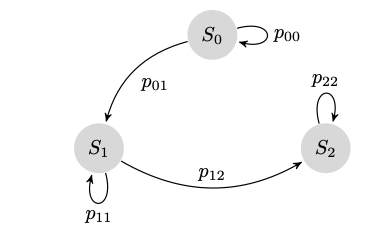
\includegraphics{figures/MarkovChain.png}

How likely is it that the system with these parameters fails during a
100h inspection interval?

The IS approach in this case is to clone ``successful'' chains,
i.e.~such that progressed to the initial failure states and simulate
these with a higher number, the so called offsprings.

As the number of offsprings is known, it is easy to correct the results
for the higher frequency of failure.

In the example below, the standard MC as well as the splitting IS
approach can be compared in a Monte Carlo simulation.

    \begin{tcolorbox}[breakable, size=fbox, boxrule=1pt, pad at break*=1mm,colback=cellbackground, colframe=cellborder]
\prompt{In}{incolor}{7}{\boxspacing}
\begin{Verbatim}[commandchars=\\\{\}]
\PY{n}{N} \PY{o}{=} \PY{l+m+mi}{100}\PY{p}{;} \PY{c+c1}{\PYZsh{} Number of repeated simulations}
\PY{n}{M} \PY{o}{=} \PY{l+m+mi}{100}\PY{p}{;} \PY{c+c1}{\PYZsh{} Number of MC samples (Length of chain)}
\PY{n}{L} \PY{o}{=} \PY{l+m+mf}{1e3}\PY{p}{;} \PY{c+c1}{\PYZsh{} Number of initial Simulations}
\PY{n}{O} \PY{o}{=} \PY{l+m+mf}{1e2}\PY{p}{;} \PY{c+c1}{\PYZsh{} Number of Offsprings}

\PY{c+c1}{\PYZsh{} Transition probability}
\PY{n}{p01} \PY{o}{=} \PY{l+m+mf}{0.001}
\PY{n}{p12} \PY{o}{=} \PY{l+m+mf}{0.0001}
\PY{c+c1}{\PYZsh{} Prepared arrays to save values}
\PY{n}{I} \PY{o}{=} \PY{n}{np}\PY{o}{.}\PY{n}{zeros}\PY{p}{(}\PY{n+nb}{int}\PY{p}{(}\PY{n}{L}\PY{p}{)}\PY{p}{)}
\PY{n}{p2} \PY{o}{=} \PY{n}{np}\PY{o}{.}\PY{n}{zeros}\PY{p}{(}\PY{n+nb}{int}\PY{p}{(}\PY{n}{N}\PY{p}{)}\PY{p}{)}
\PY{n}{p3} \PY{o}{=} \PY{n}{np}\PY{o}{.}\PY{n}{zeros}\PY{p}{(}\PY{n+nb}{int}\PY{p}{(}\PY{n}{N}\PY{p}{)}\PY{p}{)}
\PY{n}{IC} \PY{o}{=} \PY{n}{np}\PY{o}{.}\PY{n}{zeros}\PY{p}{(}\PY{n+nb}{int}\PY{p}{(}\PY{n}{O}\PY{p}{)}\PY{p}{)}
\PY{n}{pS} \PY{o}{=} \PY{n}{np}\PY{o}{.}\PY{n}{zeros}\PY{p}{(}\PY{n+nb}{int}\PY{p}{(}\PY{n}{N}\PY{p}{)}\PY{p}{)}
\PY{n}{pN} \PY{o}{=} \PY{n}{np}\PY{o}{.}\PY{n}{zeros}\PY{p}{(}\PY{n+nb}{int}\PY{p}{(}\PY{n}{N}\PY{p}{)}\PY{p}{)}
\PY{c+c1}{\PYZsh{} Repeat the MC example N times}
\PY{k}{for} \PY{n}{k} \PY{o+ow}{in} \PY{n+nb}{range}\PY{p}{(}\PY{l+m+mi}{0}\PY{p}{,}\PY{n}{N}\PY{p}{)}\PY{p}{:}
    \PY{c+c1}{\PYZsh{} Initial simulations from P0}
    \PY{k}{for} \PY{n}{i} \PY{o+ow}{in} \PY{n+nb}{range}\PY{p}{(}\PY{l+m+mi}{0}\PY{p}{,}\PY{n+nb}{int}\PY{p}{(}\PY{n}{L}\PY{p}{)}\PY{p}{)}\PY{p}{:}
        \PY{n}{Ii} \PY{o}{=} \PY{n}{np}\PY{o}{.}\PY{n}{flatnonzero}\PY{p}{(}\PY{n}{rng}\PY{o}{.}\PY{n}{uniform}\PY{p}{(}\PY{n}{size}\PY{o}{=}\PY{n}{N}\PY{p}{)} \PY{o}{\PYZlt{}} \PY{n}{p01}\PY{p}{)}
        \PY{n}{I}\PY{p}{[}\PY{n}{i}\PY{p}{]} \PY{o}{=} \PY{n+nb}{min}\PY{p}{(}\PY{n}{Ii}\PY{o}{.}\PY{n}{tolist}\PY{p}{(}\PY{p}{)}\PY{p}{,} \PY{n}{default}\PY{o}{=}\PY{n}{M}\PY{o}{+}\PY{l+m+mi}{1}\PY{p}{)}
    \PY{c+c1}{\PYZsh{} Calculate intermediate probability}
    \PY{n}{R2} \PY{o}{=} \PY{n}{np}\PY{o}{.}\PY{n}{sum}\PY{p}{(}\PY{l+m+mf}{1.0}\PY{o}{*}\PY{p}{(}\PY{n}{I} \PY{o}{\PYZlt{}} \PY{n}{M}\PY{o}{+}\PY{l+m+mi}{1}\PY{p}{)}\PY{p}{)}\PY{p}{;}
    \PY{n}{p2}\PY{p}{[}\PY{n}{k}\PY{p}{]} \PY{o}{=} \PY{n}{R2}\PY{o}{/}\PY{n}{L}\PY{p}{;}
    
    \PY{n}{N3} \PY{o}{=} \PY{l+m+mi}{0}\PY{p}{;}
    \PY{n}{R3} \PY{o}{=} \PY{l+m+mi}{0}\PY{p}{;}
    \PY{k}{for} \PY{n}{i} \PY{o+ow}{in} \PY{n+nb}{range}\PY{p}{(}\PY{l+m+mi}{0}\PY{p}{,} \PY{n+nb}{int}\PY{p}{(}\PY{n}{L}\PY{p}{)}\PY{p}{)}\PY{p}{:}
        \PY{k}{if} \PY{p}{(}\PY{n}{I}\PY{p}{[}\PY{n}{i}\PY{p}{]} \PY{o}{\PYZlt{}} \PY{n}{M}\PY{o}{+}\PY{l+m+mi}{1}\PY{p}{)}\PY{p}{:}
            \PY{k}{for} \PY{n}{j} \PY{o+ow}{in} \PY{n+nb}{range}\PY{p}{(}\PY{l+m+mi}{0}\PY{p}{,} \PY{n+nb}{int}\PY{p}{(}\PY{n}{O}\PY{p}{)}\PY{p}{)}\PY{p}{:}
                \PY{c+c1}{\PYZsh{} Clone succesful trajectories}
                \PY{n}{YC} \PY{o}{=} \PY{n}{np}\PY{o}{.}\PY{n}{flatnonzero}\PY{p}{(}\PY{n}{rng}\PY{o}{.}\PY{n}{uniform}\PY{p}{(}\PY{n}{size}\PY{o}{=}\PY{n+nb}{int}\PY{p}{(}\PY{n}{M}\PY{o}{\PYZhy{}}\PY{n}{I}\PY{p}{[}\PY{n}{i}\PY{p}{]}\PY{o}{+}\PY{l+m+mi}{1}\PY{p}{)}\PY{p}{)} \PY{o}{\PYZlt{}} \PY{n}{p12}\PY{p}{)}
                \PY{c+c1}{\PYZsh{} Check Offsprings for succesful trajectories}
                \PY{n}{IC}\PY{p}{[}\PY{n}{j}\PY{p}{]} \PY{o}{=} \PY{n+nb}{min}\PY{p}{(}\PY{n}{YC}\PY{o}{.}\PY{n}{tolist}\PY{p}{(}\PY{p}{)}\PY{p}{,} \PY{n}{default}\PY{o}{=}\PY{n}{M}\PY{o}{+}\PY{l+m+mi}{1}\PY{p}{)}\PY{p}{;}
            \PY{n}{R3} \PY{o}{=} \PY{n}{R3} \PY{o}{+} \PY{n+nb}{sum}\PY{p}{(}\PY{l+m+mf}{1.0}\PY{o}{*}\PY{p}{(}\PY{n}{IC} \PY{o}{\PYZlt{}} \PY{n}{M}\PY{o}{+}\PY{l+m+mi}{1}\PY{p}{)}\PY{p}{)}\PY{p}{;}
            \PY{n}{N3} \PY{o}{=} \PY{n}{N3} \PY{o}{+} \PY{n}{O}\PY{p}{;}
    \PY{k}{if} \PY{p}{(}\PY{n}{N3} \PY{o}{\PYZgt{}} \PY{l+m+mi}{0}\PY{p}{)}\PY{p}{:}
        \PY{n}{p3}\PY{p}{[}\PY{n}{k}\PY{p}{]} \PY{o}{=} \PY{n}{R3}\PY{o}{/}\PY{n}{N3}\PY{p}{;}
    \PY{k}{else}\PY{p}{:}
        \PY{n}{p3}\PY{p}{[}\PY{n}{k}\PY{p}{]} \PY{o}{=} \PY{l+m+mi}{0}\PY{p}{;}
    \PY{n}{nS} \PY{o}{=} \PY{l+m+mi}{0}
    \PY{c+c1}{\PYZsh{}\PYZsh{}\PYZsh{}\PYZsh{}\PYZsh{}\PYZsh{}\PYZsh{}\PYZsh{}\PYZsh{}\PYZsh{}\PYZsh{}\PYZsh{}\PYZsh{}\PYZsh{}\PYZsh{}\PYZsh{}\PYZsh{}\PYZsh{}\PYZsh{}\PYZsh{}\PYZsh{}\PYZsh{}\PYZsh{}\PYZsh{}\PYZsh{}\PYZsh{}\PYZsh{}\PYZsh{}\PYZsh{}\PYZsh{}}
    \PY{c+c1}{\PYZsh{} Standard MC of comparable length}
    \PY{k}{for} \PY{n}{m} \PY{o+ow}{in} \PY{n+nb}{range}\PY{p}{(}\PY{l+m+mi}{0}\PY{p}{,} \PY{n+nb}{int}\PY{p}{(}\PY{n}{L}\PY{o}{+}\PY{n}{N3}\PY{p}{)}\PY{p}{)}\PY{p}{:}
        \PY{n}{Ii} \PY{o}{=} \PY{n}{np}\PY{o}{.}\PY{n}{flatnonzero}\PY{p}{(}\PY{n}{rng}\PY{o}{.}\PY{n}{uniform}\PY{p}{(}\PY{n}{size}\PY{o}{=}\PY{n}{M}\PY{p}{)} \PY{o}{\PYZlt{}} \PY{n}{p01}\PY{p}{)}
        \PY{n}{I1} \PY{o}{=} \PY{n+nb}{min}\PY{p}{(}\PY{n}{Ii}\PY{o}{.}\PY{n}{tolist}\PY{p}{(}\PY{p}{)}\PY{p}{,} \PY{n}{default}\PY{o}{=}\PY{n}{M}\PY{o}{+}\PY{l+m+mi}{1}\PY{p}{)}
        \PY{n}{Ii} \PY{o}{=} \PY{n}{np}\PY{o}{.}\PY{n}{flatnonzero}\PY{p}{(}\PY{n}{rng}\PY{o}{.}\PY{n}{uniform}\PY{p}{(}\PY{n}{size}\PY{o}{=}\PY{n+nb}{int}\PY{p}{(}\PY{n}{M}\PY{o}{\PYZhy{}}\PY{n}{I1}\PY{o}{+}\PY{l+m+mi}{1}\PY{p}{)}\PY{p}{)} \PY{o}{\PYZlt{}} \PY{n}{p12}\PY{p}{)}
        \PY{n}{nS} \PY{o}{=} \PY{n}{nS} \PY{o}{+} \PY{p}{(}\PY{n+nb}{min}\PY{p}{(}\PY{n}{Ii}\PY{o}{.}\PY{n}{tolist}\PY{p}{(}\PY{p}{)}\PY{p}{,} \PY{n}{default}\PY{o}{=}\PY{n}{M}\PY{o}{+}\PY{l+m+mi}{1}\PY{p}{)} \PY{o}{\PYZlt{}} \PY{n}{M}\PY{o}{+}\PY{l+m+mi}{1}\PY{p}{)}
    \PY{n}{pS}\PY{p}{[}\PY{n}{k}\PY{p}{]} \PY{o}{=} \PY{n}{p2}\PY{p}{[}\PY{n}{k}\PY{p}{]}\PY{o}{*}\PY{n}{p3}\PY{p}{[}\PY{n}{k}\PY{p}{]}
    \PY{n}{pN}\PY{p}{[}\PY{n}{k}\PY{p}{]} \PY{o}{=} \PY{n}{nS}\PY{o}{/}\PY{p}{(}\PY{n}{L}\PY{o}{+}\PY{n}{N3}\PY{p}{)}

\PY{c+c1}{\PYZsh{} Plotting}
\PY{n}{plt}\PY{o}{.}\PY{n}{figure}\PY{p}{(}\PY{n}{figsize}\PY{o}{=}\PY{p}{(}\PY{l+m+mi}{6}\PY{p}{,}\PY{l+m+mi}{8}\PY{p}{)}\PY{p}{)}
\PY{n}{plt}\PY{o}{.}\PY{n}{subplot}\PY{p}{(}\PY{l+m+mi}{211}\PY{p}{)}
\PY{n}{plt}\PY{o}{.}\PY{n}{hist}\PY{p}{(}\PY{n}{pN}\PY{p}{,} \PY{n}{label}\PY{o}{=}\PY{l+s+s2}{\PYZdq{}}\PY{l+s+s2}{Standard MC}\PY{l+s+s2}{\PYZdq{}}\PY{p}{)}
\PY{n}{plt}\PY{o}{.}\PY{n}{legend}\PY{p}{(}\PY{p}{)}
\PY{n}{plt}\PY{o}{.}\PY{n}{subplot}\PY{p}{(}\PY{l+m+mi}{212}\PY{p}{)}
\PY{n}{plt}\PY{o}{.}\PY{n}{hist}\PY{p}{(}\PY{n}{pS}\PY{p}{,} \PY{n}{label}\PY{o}{=}\PY{l+s+s2}{\PYZdq{}}\PY{l+s+s2}{Importance Sampling}\PY{l+s+s2}{\PYZdq{}}\PY{p}{)}
\PY{n}{plt}\PY{o}{.}\PY{n}{legend}\PY{p}{(}\PY{p}{)}

\PY{n+nb}{print}\PY{p}{(}\PY{l+s+s2}{\PYZdq{}}\PY{l+s+s2}{Splitting: }\PY{l+s+s2}{\PYZdq{}}\PY{p}{,} \PY{n}{np}\PY{o}{.}\PY{n}{mean}\PY{p}{(}\PY{n}{pS}\PY{p}{)}\PY{p}{,} \PY{l+s+s2}{\PYZdq{}}\PY{l+s+s2}{ +/\PYZhy{} }\PY{l+s+s2}{\PYZdq{}}\PY{p}{,} \PY{n}{np}\PY{o}{.}\PY{n}{std}\PY{p}{(}\PY{n}{pS}\PY{p}{)}\PY{p}{)}
\PY{n+nb}{print}\PY{p}{(}\PY{l+s+s2}{\PYZdq{}}\PY{l+s+s2}{Standard:  }\PY{l+s+s2}{\PYZdq{}}\PY{p}{,} \PY{n}{np}\PY{o}{.}\PY{n}{mean}\PY{p}{(}\PY{n}{pN}\PY{p}{)}\PY{p}{,} \PY{l+s+s2}{\PYZdq{}}\PY{l+s+s2}{ +/\PYZhy{} }\PY{l+s+s2}{\PYZdq{}}\PY{p}{,} \PY{n}{np}\PY{o}{.}\PY{n}{std}\PY{p}{(}\PY{n}{pN}\PY{p}{)}\PY{p}{)}
\PY{n+nb}{print}\PY{p}{(}\PY{l+s+s2}{\PYZdq{}}\PY{l+s+s2}{Variance Reduction: }\PY{l+s+s2}{\PYZdq{}}\PY{p}{,} \PY{p}{(}\PY{n}{np}\PY{o}{.}\PY{n}{std}\PY{p}{(}\PY{n}{pN}\PY{p}{)}\PY{o}{/}\PY{n}{np}\PY{o}{.}\PY{n}{std}\PY{p}{(}\PY{n}{pS}\PY{p}{)}\PY{p}{)}\PY{p}{)}
\PY{n+nb}{print}\PY{p}{(}\PY{l+s+s2}{\PYZdq{}}\PY{l+s+s2}{Offsprings: }\PY{l+s+s2}{\PYZdq{}}\PY{p}{,} \PY{p}{(}\PY{n}{np}\PY{o}{.}\PY{n}{mean}\PY{p}{(}\PY{n}{N3}\PY{p}{)}\PY{p}{)}\PY{p}{)}
\end{Verbatim}
\end{tcolorbox}

    \begin{Verbatim}[commandchars=\\\{\}]
Splitting:  0.0005064999999999999  +/-  8.539759949787816e-05
Standard:   0.0005361265817386119  +/-  0.00019924415331549634
Variance Reduction:  2.3331352928772535
Offsprings:  8500.0
    \end{Verbatim}

    \begin{center}
    \adjustimage{max size={0.9\linewidth}{0.9\paperheight}}{output_15_1.png}
    \end{center}
    { \hspace*{\fill} \\}
    
    \hypertarget{exercise}{%
\subsection{Exercise}\label{exercise}}

Try different parameters in the simulation example, e.g.~for the number
of offsprings or the transition probabilities. What do you observe?

Careful: simulation times may get long!

    \begin{tcolorbox}[breakable, size=fbox, boxrule=1pt, pad at break*=1mm,colback=cellbackground, colframe=cellborder]
\prompt{In}{incolor}{ }{\boxspacing}
\begin{Verbatim}[commandchars=\\\{\}]

\end{Verbatim}
\end{tcolorbox}


    % Add a bibliography block to the postdoc
    
    
    
\end{document}
